%%%%%%%%%%%%%%%%%%%%%%%%%%%%%%%%%%%%%%%%%%%%%%%%%%%%%%%%%%%%%%%%%%%%%%%%%%%%%%%%
%2345678901234567890123456789012345678901234567890123456789012345678901234567890
%        1         2         3         4         5         6         7         8

%\documentclass[letterpaper, 10 pt, conference]{ieeeconf}  % Comment this line out
                                                          % if you need a4paper
\documentclass[a4paper, 10pt, conference]{ieeeconf}      % Use this line for a4
                                                          % paper

\IEEEoverridecommandlockouts                              % This command is only
                                                          % needed if you want to
                                                          % use the \thanks command
\overrideIEEEmargins
% See the \addtolength command later in the file to balance the column lengths
% on the last page of the document

\usepackage{graphicx}
\usepackage[margin=1in]{geometry}
\usepackage{hyperref}
\usepackage{amsmath}
\usepackage{mathrsfs}
\usepackage{float}

\DeclareMathOperator{\card}{card}
\DeclareMathOperator{\trc}{trace}
\DeclareMathOperator{\mean}{mean}
\DeclareMathOperator{\bin}{bin}
\DeclareMathOperator{\lns}{lanes}
\DeclareMathOperator{\cnt}{count}

\bibliographystyle{ieeetr}

% The following packages can be found on http:\\www.ctan.org
%\usepackage{graphics} % for pdf, bitmapped graphics files
%\usepackage{epsfig} % for postscript graphics files
%\usepackage{mathptmx} % assumes new font selection scheme installed
%\usepackage{times} % assumes new font selection scheme installed
%\usepackage{amsmath} % assumes amsmath package installed
%\usepackage{amssymb}  % assumes amsmath package installed

\title{\LARGE \bf
Linearized Aw-Rascle-Zhang Model for Road Traffic Prediction and Control
}

%\author{ \parbox{3 in}{\centering Huibert Kwakernaak*
%         \thanks{*Use the $\backslash$thanks command to put information here}\\
%         Faculty of Electrical Engineering, Mathematics and Computer Science\\
%         University of Twente\\
%         7500 AE Enschede, The Netherlands\\
%         {\tt\small h.kwakernaak@autsubmit.com}}
%         \hspace*{ 0.5 in}
%         \parbox{3 in}{ \centering Pradeep Misra**
%         \thanks{**The footnote marks may be inserted manually}\\
%        Department of Electrical Engineering \\
%         Wright State University\\
%         Dayton, OH 45435, USA\\
%         {\tt\small pmisra@cs.wright.edu}}
%}

\author{Francois Belletti, Mandy Huo, Xavier Litrico, Alexandre M. Bayen}

\begin{document}

\maketitle
\thispagestyle{empty}
\pagestyle{empty}

\begin{abstract}
This article starts from the classical Aw-Rascle-Zhang (ARZ) model for freeway traffic and develops a spectral analysis of its linearized version. A counterpart to the Froude number in hydrodynamics is defined that enables a classification of the nature of vehicle traffic flow using the explicit solution resulting from the analysis. We prove that our linearization about an equilibrium is stable for congested regimes and unstable otherwise. NGSIM data for congested traffic trajectories is used so as to confront the linearized model's predictions to actual macroscopic behavior of traffic. The model is shown to achieve good accuracy for speed and flow. In particular, it replicates the propagation of boundary conditions' oscillations into the interior resolution domain of the PDE under study.
\end{abstract}

%\linenumbers

\section{Introduction}

In traffic control and data mining communities, non-linearity most of the time presents challenges when it comes to devising control strategies or applying estimation theory. Empirical studies of goodness of fit would usually have researchers elect non-linear first order models such as LWR [CITE] or non-linear second order models such as [CITE]. [REPHRASE].

In that regard, second order models such as PW [CITE] where first presented as a compelling opportunity to account for many features empirically observed in traffic such as .... . Although Daganzo highlighted many flaws of the first generation of that family of models, a second generation offered a step towards more realism in macroscopic traffic modeling. Talk about good properties of ARZ, a word about phase transition models. [REPHRASE]

Unfortunately, mathematical properties such as the inf-morphism principle [CITE CLAUDEL, BLANDIN, HOFTLEINER] have not found straightforward analogs in bi-variate second order models. The non-linearity of these models is therefore a strong challenge when it comes to devising control and data assimilation strategies with such models. [REPHRASE]

ARZ features phenomena of persisting linear oscillations that an accurate model for traffic is expected to account for. Similarly, traffic instability has been observed in practice and gave rise to many theoretical studies (Jamitons). Linearizing the ARZ model, based on the work of Litrico, offers a compelling opportunity to work in a realistic modeling framework where the phenomena mentioned above are present and, at the same time, use linear control theory and spectral Laplace analysis. [REPHRASE]

Our approach in this paper is therefore to linearize the ARZ model about an equilibrium so as to make the best of a trade-off between model accuracy and ease of use. The first section is dedicated to the linearization and spectral analysis of the ARZ model. We prove there is convective instability in free-flow regime that drives the model away from its equilibrium and devise an equivalent of the hydrodynamics' Fraud number for traffic macroscopic models. Laplace transforms and low frequency analysis also present many properties whose interpretation is tractable and simple. The second section focuses on the accuracy of the model. It confronts its predictions with ground truth data extracted from the NGSIM data with [GIVE CHARACTERISTICS OF DATA SET]. It also shows how to leverage spectral analysis so as to compute traffic prediction without the need for finite difference or Riemann based numerical schemes. [REPHRASE]

\section{The ARZ model} \label{ARZSection}

%\begin{itemize}
%\item physical description of ARZ model + usual form
%\item $(v, q)$ form, well-posedness 
%\end{itemize}

We consider the ARZ model with relaxation term. The model is shown here: 
\begin{align} 
\rho_t + (\rho v)_x &= 0, \label{ARZ1} \\
(v - V(\rho))_t + v(v - V(\rho))_x &=\dfrac{V(\rho) - v}{\tau} \label{ARZ2},
\end{align}
where $\rho$ is the density, $v$ is the velocity, $\tau$ is the relaxation time, and $V(\rho) = Q(\rho)/\rho$ is the equilibrium velocity profile, where $Q(\rho)$ is the density-flow relation given by the fundamental diagram. We assume that $V$ is $C^{1}$ derivable over its domain. Without the relaxation term cars never reach the maximum allowable speed \cite{R_improved} and the steady-state relation between density and speed is broken in the presence of road junctions \cite{jin2015}. Note that at the equilibrium velocity this term is zero. 

In vector form the ARZ model is
\begin{equation} \label{ARZrhov}
\begin{pmatrix}
	\rho \\
	v
\end{pmatrix}_t
+ 
C_1 \left(\rho, v \right)
\begin{pmatrix}
	\rho \\ 
	v
\end{pmatrix}_x = 
\begin{pmatrix}
	0 \\ 
	\dfrac{V(\rho) - v}{\tau}
\end{pmatrix}.
\end{equation}

where

\begin{equation}
C_1 \left( \rho, v \right) =
\begin{pmatrix}
	v & \rho \\
	0 & v + \rho V' (\rho)
\end{pmatrix}
\end{equation}

With the appropriate variable change, we can rewrite the model in the density-flow and velocity-flow forms, the latter of which is most useful to us for practical control purposes. Using the flow relation $q = \rho v$ and \eqref{ARZrhov}, the density-flow form is

\begin{align}
\begin{pmatrix}
	\rho \\
	q
\end{pmatrix}_t 
+
C_2\left(\rho, q\right)
\begin{pmatrix}
	\rho \\ 
	q
\end{pmatrix}_t
&=
\begin{pmatrix}
	0 \\ 
	\frac{Q(\rho) - q}{\tau}
\end{pmatrix}. \label{ARZrhoq}  \\
\begin{pmatrix}
	v \\ 
	q
\end{pmatrix}_t
+ C_3\left(v, q\right)
\begin{pmatrix}
	v \\ 
	q
\end{pmatrix}_x 
&= 
\dfrac{1}{\tau}
\begin{pmatrix}
	V\left( \frac{q}{v}\right) - v \\
	Q\left( \frac{q}{v}\right) - q
\end{pmatrix}.
\label{ARZrhov}
\end{align}

where

\begin{align}
C_2 \left(\rho, q \right)
&= 
\begin{pmatrix}
	0 & 1 \\
	- \frac{q}{\rho} \left( \frac{q}{\rho} + \rho V'\left( \rho \right) \right) & 2 \frac{q}{\rho} + \rho V'\left( \rho \right) \\
\end{pmatrix} \\
C_3 \left(v, q \right)
&=
\begin{pmatrix}
	v + \frac{q}{v} V'\left( \frac{q}{v} \right) & 0 \\
	\frac{q}{v} \left( v + \frac{q}{v} V'\left( \frac{q}{v} \right) \right) & v
\end{pmatrix}
\end{align}

It is noteworthy that \ref{ARZrhoq} is equivalent to the conservative form

\begin{equation}
\begin{pmatrix}
	\rho \\ 
	q - Q \left( \rho \right)
\end{pmatrix}_t
+
\begin{pmatrix}
	q \\ 
	\frac{q}{\rho} \left( q - Q \left( \rho \right) \right)
\end{pmatrix}_x =
\begin{pmatrix}
	0 \\
	\frac{Q\left( \rho \right) - q}{\tau}
\end{pmatrix}
\end{equation}

most helpful in \cite{Piccoli201532} and \cite{Delis2014318} for data assimilation and macroscopic traffic simulation respectively.

The $\left(v, q \right)$ form has seldom been used in transportation engineering however it is promising for data fusion purposes that involve both loop detector measurements (providing values for $q$) and GPS traces (giving estimates for $v$).


\subsection{Linearization}
We are interested in small deviations, $(\tilde{\rho}(x,t), \tilde{v}(x,t))$, from a given nominal profile. Consider the nominal solution $(\rho^*(x),v^*(x))(V(\rho^*) = v^*)$ satisfying $v_t = \rho_t = 0$. Then \eqref{ARZrhov} becomes
\begin{align}
v^* \rho^*_x + v^*_x\rho^* = 0, \\
( v^* + \rho^* V'( \rho^*) )v^*_x = \dfrac{V(\rho^*) - v^*}{\tau} = 0.
\end{align}
Then we must have $v^*_x=\rho^*_x=0$, so the solution is uniform along the road. 

Linearizing the ARZ model \eqref{ARZrhov} around the nominal solution described above, we obtain
\begin{align} \label{rhovlin}
\begin{pmatrix}
	\tilde{\rho} \\
	\tilde{v}
\end{pmatrix}_t
+ \bar{C}_1
\begin{pmatrix}
	\tilde{\rho} \\ 
	\tilde{v}
\end{pmatrix}_x 
&= 
\bar{B}_1
\begin{pmatrix}
	\tilde{\rho} \\
	\tilde{v}
\end{pmatrix}.
\\
\end{align}

where

\begin{align}
\bar{C}_1 &= 
\begin{pmatrix}
	v^* & \rho^* \\
	0 & v^* + \rho^* V' ( \rho^*) 
\end{pmatrix} \\
\bar{B}_1 &= 
-\frac{1}{\tau}
\begin{pmatrix}
	0 & 0 \\
	V'\left( \rho^{*} \right) & -1
\end{pmatrix}
\end{align}

Similarly, for the density-flow system \eqref{ARZrhoq} we linearize around the equilibrium $(\rho^*, q^*)(\rho^*V(\rho^*) = q^*)$ with deviations $(\tilde{\rho}(x,t), \tilde{q}(x,t))$.The analogs of $\bar{C}_1$ and $\bar{B}_1$ are denoted $\bar{C}_2$ and $\bar{B}_2$ in \ref{eq:C2} and \ref{eq:C3}. For the deviations $(\tilde{v}, \tilde{q})$ from the equilibrium we adopt similar notations with $\bar{C}_3$ and $\bar{B}_3$ given in \ref{eq:C3} and \ref{eq:B3}. This last form, most adapted to traffic prediction and control in practical settings where flows and vehicle velocities are measured will be studied in what follows.

\begin{align}
\bar{C}_2 &= \label{eq:C2}
\begin{pmatrix}
	0 & 1 \\
	-\frac{q^{*}}{\rho{*}} \left(
		\frac{q^{*}}{\rho{*}} + \rho^{*} V'\left( \rho^{*} \right) \right) & 2 \frac{q^{*}}{\rho^{*}} + \rho^{*} V'\left( \rho^{*} \right)
\end{pmatrix} \\
\bar{B}_2 &= \label{eq:B2}
\frac{1}{\tau}
\begin{pmatrix}
	0 & 0 \\
	V'\left( \rho^{*} \right) & -1
\end{pmatrix} \\
\bar{C}_3 &= \label{eq:C3}
\begin{pmatrix}
	v^* + \frac{q^*}{v^*} V'\left(\frac{q^*}{v^*}\right) & 0 \\
	\frac{q^*}{v^*} \left( v^* + \frac{q^*}{v^*} V'\left(\frac{q^*}{v^*}\right)\right) & v^*
\end{pmatrix} \\
\bar{B}_3 &= \label{eq:B3}
\frac{1}{v^{*}\tau}
\begin{pmatrix}
		-\dfrac{(v^*)^2+q^*V'\left(\frac{q^*}{v^*}\right)}{v^*} & V'\left(\frac{q^*}{v^*}\right) \\
		-\dfrac{q^*\left((v^*)^2 + q^*V'\left(\frac{q^*}{v^*}\right)\right)}{(v^*)^2}  & \dfrac{q^*V'\left(\frac{q^*}{v^*}\right)}{v^*}
\end{pmatrix} \\
\end{align}




\subsection{Characteristic form}
We diagonalize the linearized equations to obtain a more useful form of the model, which will then be treated in the spectral domain. 
%We can rewrite \eqref{rhovlin} in diagonal form. The eigenvalues of $A$ are 
%\begin{align}
%\lambda_1 &= v^*, \\
%\lambda_2 &= v^* + \rho^* V'( \rho^*).
%\end{align}
We begin with the density-flow system. Standard algebraic manipulations of the equations in \eqref{rhovlin} lead to
\begin{equation}
\begin{pmatrix}
\xi_1 \\ \xi_2
\end{pmatrix}_t
+ \begin{pmatrix}
\lambda_1 & 0 \\
0 & \lambda_2 
\end{pmatrix}
\begin{pmatrix}
\xi_1 \\ \xi_2
\end{pmatrix}_x
= \begin{pmatrix}
-\frac{1}{\tau} & 0 \\
-\frac{1}{\tau} & 0
\end{pmatrix}
\begin{pmatrix}
\xi_1 \\ \xi_2
\end{pmatrix},
\end{equation}
where $\xi_1 = \tilde{v} - V'( \rho^* )\tilde{\rho}$ and $\xi_2 = \tilde{v}$ are the Riemann invariants of the $(\rho, v)$ system, and $\lambda_1 = v^*$ and $\lambda_2 = v^* + \rho^* V'( \rho^*)$ are the eigenvalues. Note that $V'( \rho^*) \leq 0$ so $\lambda_2 \leq \lambda_1 = v^*$. Therefore this is consistent with the physical dynamics of the system as no waves travel faster than the equilibrium vehicle speed. 

We proceed in the same manner as above to diagonalize the $(\rho,q)$ system \eqref{rhoqlin}. The diagonal form is
\begin{equation} \label{rhoqlindiag}
\begin{pmatrix}
\chi_1 \\ \chi_2
\end{pmatrix}_t 
+ \begin{pmatrix}
\lambda_1 & 0 \\
0 & \lambda_2
\end{pmatrix}
\begin{pmatrix}
\chi_1 \\ \chi_2
\end{pmatrix}_x
= \begin{pmatrix}
-\frac{1}{\tau} & 0 \\
-\frac{1}{\tau} & 0
\end{pmatrix}
\begin{pmatrix}
\chi_1 \\ \chi_2
\end{pmatrix},
\end{equation}
where $\chi_1 = -\lambda_2 \tilde{\rho} + \tilde{q}$ and $\chi_2 = -\lambda_1 \tilde{\rho} + \tilde{q}$ are the characteristic variables in the $(\rho,q)$ system and the eigenvalues $\lambda_1$ and $\lambda_2$ are the same as in the density-velocity system due to the relation $q^* = \rho^*v^*$. 

Diagonalization of the velocity-flow system is more involved. Letting $\eta(x,t) = (\tilde{v}, \tilde{q})^T$, we can rewrite \eqref{vqlin} as
\begin{equation} \label{vqlinxi}
\eta_t + A\eta_x = B\eta.
\end{equation}
The eigenvalues of $A$ are $\lambda_1 = v^*$ and $\lambda_2 = v^* + \frac{q^*}{v^*} V'\left(\frac{q^*}{v^*}\right)$, consistent with the previous systems. Then $A$ can be diagonalized as follows
\begin{align}
A &= XDX^{-1}, \\
X &= \begin{pmatrix}
0 & \lambda_2-\lambda_1 \\
1 & \rho^*\lambda_2
\end{pmatrix}, \\
D &= \begin{pmatrix}
\lambda_1 & 0 \\
0 & \lambda_2
\end{pmatrix},\\
X^{-1} &= \begin{pmatrix}
\dfrac{\rho^*\lambda_2}{\lambda_1 - \lambda_2} & 1 \\
-\dfrac{1}{\lambda_1 - \lambda_2} & 0
\end{pmatrix}.
\end{align}

Define $\gamma(x,t) := X\eta(x,t)$. Hence \eqref{vqlinxi} can be rewritten as
\begin{equation} 
\gamma_t + \begin{pmatrix}
\lambda_1 & 0 \\
0 & \lambda_2
\end{pmatrix} \gamma_x = \begin{pmatrix}
-\frac{1}{\tau} & 0 \\
-\frac{1}{q^* \tau} & 0
\end{pmatrix} \gamma
\end{equation}
where 
\begin{equation}
\gamma = \begin{pmatrix}
\frac{\rho^*\lambda_2}{\lambda_1 - \lambda_2}\tilde{v} + \tilde{q} \\ 
-\frac{1}{\lambda_1 - \lambda_2}\tilde{v} 
\end{pmatrix}. 
\end{equation}

Let $\xi = (\xi_1, \xi_2)^T = (\chi_1, -q^*\chi_2)^T$. Then we have
\begin{equation} \label{vqlindiag}
\begin{pmatrix}
\xi_1 \\ \xi_2
\end{pmatrix}_t + 
\underset{\tilde{A}}{
	\underbrace{
	\begin{pmatrix}
		\lambda_1 & 0 \\
		0 & \lambda_2
	\end{pmatrix} 
	}
}
\begin{pmatrix}
\xi_1 \\ \xi_2
\end{pmatrix}_x = 
\underset{\tilde{B}}{
	\underbrace{
	\begin{pmatrix}
		-\frac{1}{\tau} & 0 \\
		-\frac{1}{\tau} & 0
	\end{pmatrix}}
}
\begin{pmatrix}
\xi_1 \\ \xi_2
\end{pmatrix},
\end{equation}
and
\begin{equation} \label{eq:Riemannzeta}
\begin{pmatrix}
\xi_1 \\ \xi_2
\end{pmatrix} = \begin{pmatrix}
\dfrac{\rho^*\lambda_2}{\lambda_1 - \lambda_2}\tilde{v} + \tilde{q} \\ 
\dfrac{q^*}{\lambda_1 - \lambda_2}\tilde{v} 
\end{pmatrix} = 
\underset{R}{
\underbrace{
	\begin{pmatrix}
		\dfrac{\rho^*\lambda_2}{\lambda_1-\lambda_2} & 1\\
		\dfrac{\rho^*\lambda_1}{\lambda_1-\lambda_2} & 0
	\end{pmatrix}
	}
}
\begin{pmatrix}
	\tilde{v} \\ \tilde{q} 
\end{pmatrix}
\end{equation}

\subsection{The Traffic Froude Number}
In fluid mechanics, the Froude number is a dimensionless number which delineates the boundary between flow regimes \cite{Sturm, litrico2009modeling}. Using the eigenvalues of the system in the characteristic form, we are able to define a useful counterpart to this number.
Since $V(\rho)$ is non-increasing function, we have $V'(\rho^*) \leq 0$. Assuming $V'(\rho^*) \neq 0$ there are two flow regimes: one in which $\lambda_1 \lambda_2 < 0$ and one characteristic line travels downstream whereas the other characteristic line travels upstream, and one in which $\lambda_1 \lambda_2 > 0$ and both characteristic lines travel downstream.

We define the \textit{Traffic Froude Number} (TFN) as
\begin{equation}
F = \left\lvert\dfrac{\rho^*V'( \rho^*)}{v^*}\right\rvert.
\end{equation} 
Then we have
\begin{equation*}
\begin{cases}
F > 1 &\Rightarrow |\rho^*V'(\rho^*)| > v^* \quad \Rightarrow \lambda_2  <0 \\
F < 1 &\Rightarrow |\rho^*V'(\rho^*)| < v^* \quad \Rightarrow \lambda_2 > 0
\end{cases}.
\end{equation*}
Note also that $\lambda_2 = v^* + \rho^* V'( \rho^*) = \dfrac{Q(\rho^*)}{\rho^*} + \dfrac{\rho^*Q'(\rho^*)-Q(\rho^*)}{\rho^*} = Q'(\rho^*)$. Hence the system is in free-flow when $F<1$ and congestion when $F>1$. In hydrodynamics these regimes are referred to as the subcritical and supercritical regimes, respectively \cite{litrico2009modeling}. The direction of characteristic lines is illustrated in Figure \ref{Characteristics}.

For traffic, the interpretation of the different regimes is somewhat different. Free flow regime corresponds to these situations where drivers are not slowed down by heavy traffic and go as fast as the desired speed. The congested regime arises when traffic is denser and, because too many cars are present on the same freeway section, drivers slow down and eventually form traffic jam.

\begin{figure}
\begin{centering}
\begin{tabular}{cc}
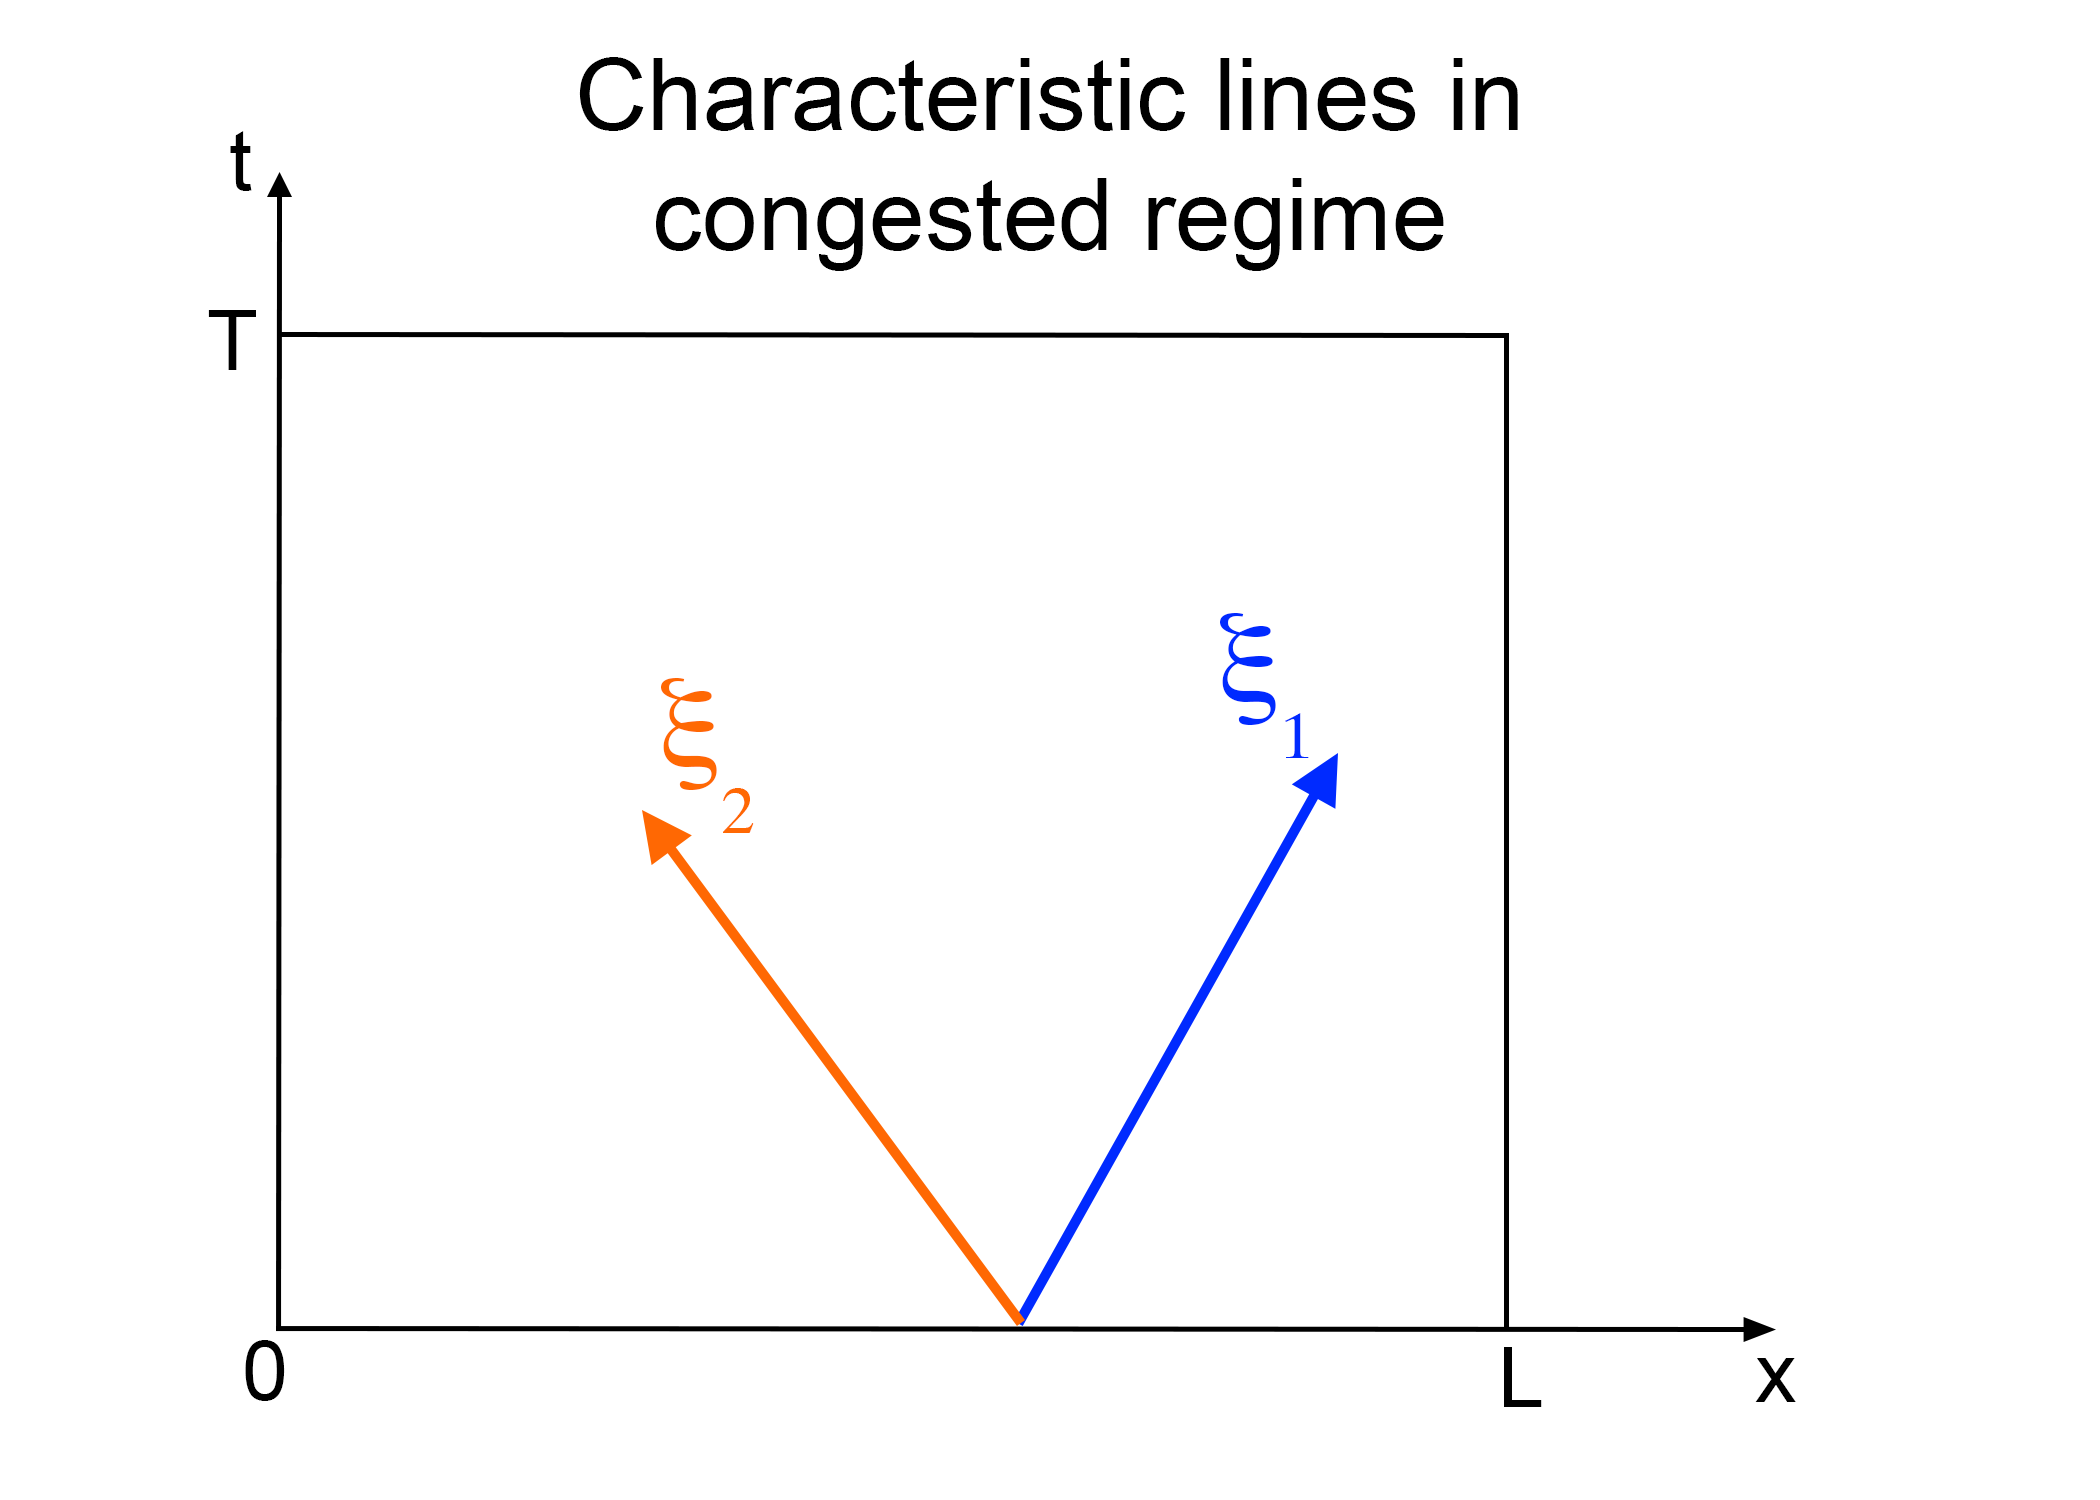
\includegraphics[width=4cm]{Congested-regime} & 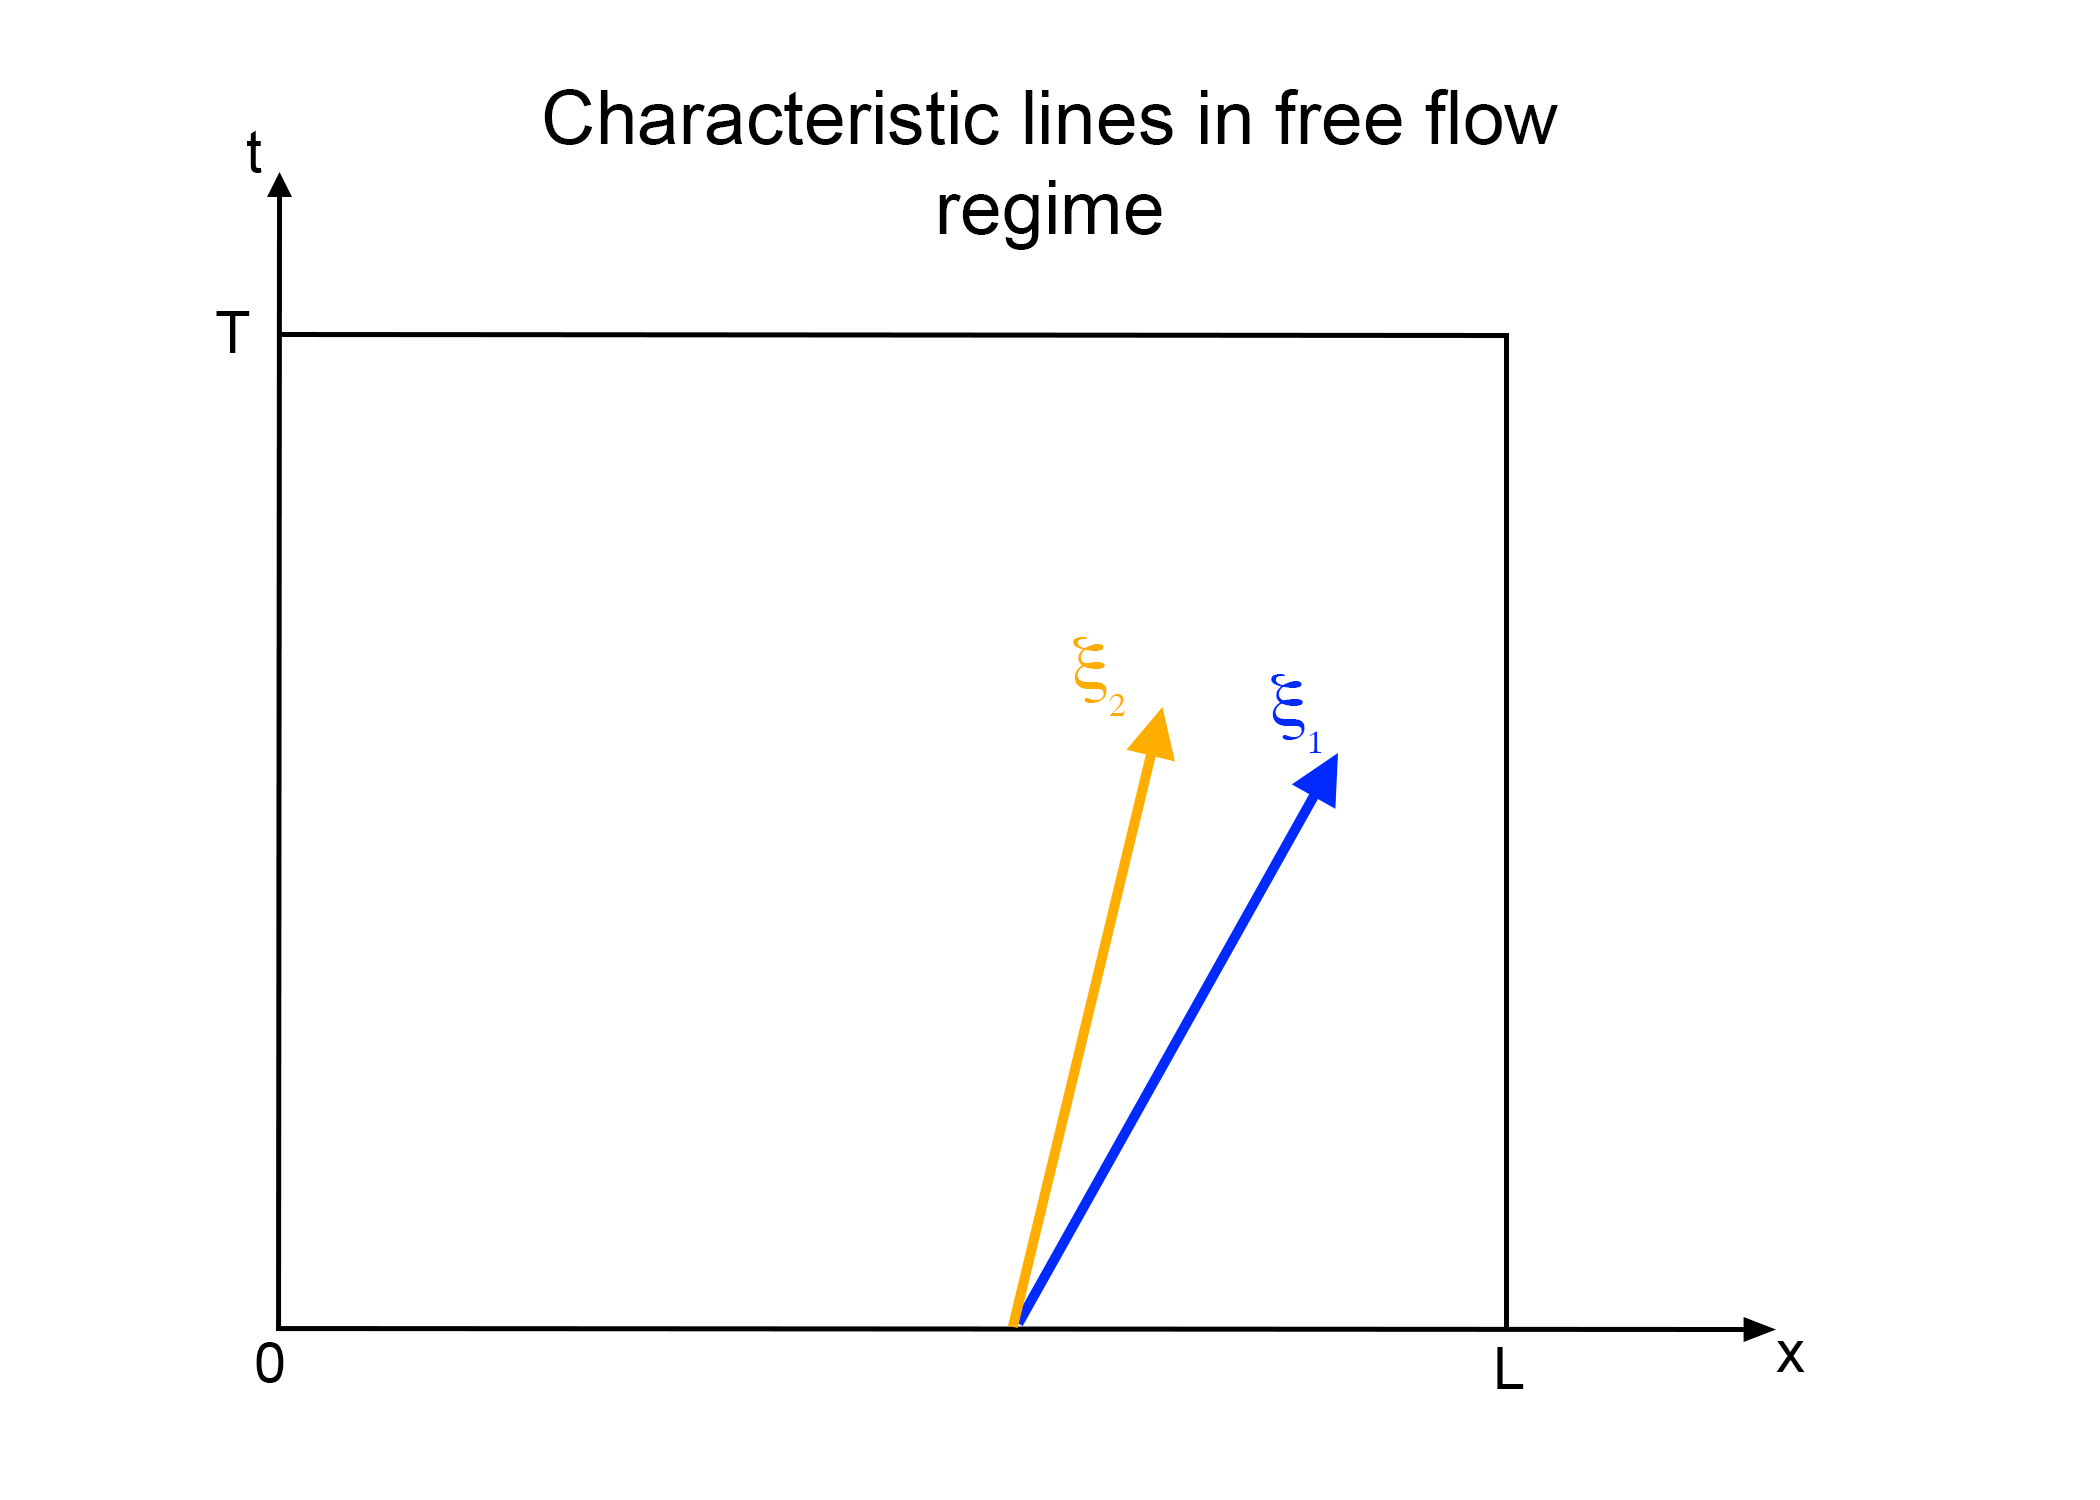
\includegraphics[width=4cm]{Free-flow-regime}\tabularnewline
$F>1$, $\lambda_{2}<0$, $\lambda_{1}>0$ & $F<1$, $\lambda_{1}>\lambda_{2}>0$\tabularnewline
\end{tabular}
\par\end{centering}
\protect\caption{Illustration of characteristic lines in congested (supercritical) and free-flow regime (subcritical) $\xi_1$ and $\xi_2$ propagate along.\label{Characteristics}}
\end{figure}


\section{Spectral analysis of the linearized ARZ model}
We now consider the $(v,q)$ system for the frequency domain analysis for practical control purposes.

\subsection{State-transition matrix}
Taking the Laplace transform of the diagonalized form \eqref{vqlindiag} we obtain 
\begin{equation}
\dfrac{\partial \hat{\xi} (x,s)}{\partial x} = \mathscr{A}(s)\hat{\xi}(x,s) + \mathscr{B}\xi(x,t=0^-),
\end{equation}
where $\mathscr{A}(s) = \tilde{A}^{-1}(\tilde{B} - sI)$ and $\mathscr{B} = -\tilde{A}^{-1}$. 

Assuming zero initial conditions we have 
\begin{equation} \label{TFRiemann}
\hat{\xi}(x,s) = \Phi(x,s)\hat{\xi}(0,s).
\end{equation}
where $\Phi(x,s) = e^{\mathscr{A}(s)x}$ is the state-transition matrix.

To compute the exponential we diagonalize the matrix $\mathscr{A}(s)$
which then yields the components of $\Phi(x,s)$:
\begin{subequations} \label{TFv0q0tovxqx}
\begin{align}
\phi_{11}(x,s) &= e^{-\frac{x}{\tau \lambda_1}}e^{-\frac{x}{\lambda_1}s}, \\ 
\phi_{12}(x,s) &= 0, \\
\phi_{21}(x,s) &= \dfrac{\lambda_1 \left( e^{-\frac{x}{\tau \lambda_1}}e^{-\frac{x}{\lambda_1}s} - e^{-\frac{x}{\lambda_2}s}\right)}{\lambda_2 - \tau (\lambda_1 - \lambda_2)s}, \\
\phi_{22}(x,s) &= e^{-\frac{x}{\lambda_2}s}.
\end{align}
\end{subequations}


Let $\alpha = -\dfrac{\lambda_2}{\tau(\lambda_1 - \lambda_2)}$. It is clear that $\phi_{11}\left(x,s\right)$ is composed of the product of a distributed delay corresponding to information propagating at speed $\lambda_{1}$ and an exponential attenuation where $\tau\lambda_{1}$ plays the role of a characteristic spatial length. Similarly $\phi_{22}$ is a delay corresponding to information propagating at speed $\lambda_{2}$. The interpretation of $\phi_{21}$ is more difficult. In low frequencies ($\left|s\right|\ll\left|\alpha\right|$), this transfer function takes a much more transparent form. Indeed, in the expression
$
\phi_{21}(x,s) = 
-\frac{\lambda_{1}}{\lambda_{2}}\frac{\alpha}
{s + \alpha}
e^{-\frac{x}{\lambda_2}s}
	\left(
		1 - e^{-\frac{x}{\lambda_1 \tau \alpha}\left(s + \alpha\right)}
	\right)
\simeq 
- \frac{\lambda_{1}}{\lambda_{2}} e^{-\frac{x}{\lambda_2}s}
	\left(
		1 - e^{-\frac{x}{\lambda_1 \tau}}
	\right)
$
the transfer function appears as the combination of a distributed delay where $\lambda_{2}$ is the propagation speed and a distributed gain where $\lambda_{1}\tau$ is a characteristic distance.

\subsection{Free-flow case ($F<1$)}
Consider the system in the free-flow regime. 

With $\xi_1 (0,t)$ and $\xi_2 (0,t)$ as the inputs and $\xi_1(L,t)$ and $\xi_2(L,t)$ as the outputs, the distributed transfer matrix is exactly the state-transition matrix $\Phi(x,s)$.\\

Using \eqref{eq:Riemannzeta}, we can write

\begin{equation} \label{vqfreeflow}
\begin{pmatrix}
	\widetilde{v}(x,s) \\ 
	\widetilde{q}(x,s)
\end{pmatrix} = 
\Psi(x,s)
\begin{pmatrix}
	\widetilde{v}(0,s) \\ 
	\widetilde{q}(0,s)
\end{pmatrix}
\end{equation}
with
\begin{subequations}
\begin{align}
\psi_{11}(x,s) &= 
\frac{
	\alpha e^{-\frac{x}{\lambda_{1}}\left(s+\frac{1}{\tau}\right)}
		+ s e^{-\frac{sx}{\lambda_{2}}}
}{
	s + \alpha
}, \\
\psi_{12}(x,s) &=
\frac{1}{\rho^* \tau}
\frac{
	e^{-\frac{sx}{\lambda_{2}}}
	-
	e^{-\frac{x}{\lambda_{1}}\left(s+\frac{1}		{\tau}\right)}
}{
	s + \alpha
}, \\
\psi_{21}(x,s) &=
- s \rho^{*} \tau \alpha
\frac{
	e^{-\frac{sx}{\lambda_{2}}}
	-
	e^{-\frac{x}{\lambda_{1}}\left(s+\frac{1}		{\tau}\right)}
}{
	s + \alpha
}, \\
\psi_{22}(x,s) &=
\frac{
	s e^{-\frac{x}{\lambda_{1}}\left(s+\frac{1}{\tau}\right)}
		+ \alpha e^{-\frac{sx}{\lambda_{2}}}
}{
	s + \alpha
}.
\end{align}
\end{subequations}

It could appear at first sight that $-\alpha$ (here a positive real) is a singularity of the transfer functions and the system is not bounded-input/bounded-output stable. However, we have $\frac{1}{\lambda_{1}}\left(-\alpha+\frac{1}{\tau}\right)=\frac{1}{\tau\left(\lambda_{1} - \lambda_{2}\right)}=\frac{-\alpha}{\lambda_{2}}$, thus a Taylor expansion about $-\alpha$ shows that numerators and denominators cancel each other out for $s \rightarrow -\alpha$. It follows that $-\alpha$ is not a pole of any transfer function. This proves that the output remains bounded for a given value of $x$. We will show below that a conic region of the $\left[0,T\right] \times \left[0,L\right]$ domain features exponential growth in free-flow regime. This arises when changing $t$ and $x$ simultaneously and complements the conclusion formulated above (in which $t$ varies and $x$ remains constant).

\subsubsection{Low frequency approximation for physical variables in free-flow regime}
Analyzing the expressions above becomes easier when approximating them for $\left|s\right|\ll\left|\alpha\right|$. This corresponds to traffic flow varying slowly and smoothly. We find the following approximate expressions for the transfer functions:
\begin{subequations}
\begin{align}
\psi_{11}(x,s)
&\simeq
e^{-\frac{sx}{\lambda_{2}}}
e^{-\frac{x}{\tau\lambda_{1}}}
, \\
\psi_{12}(x,s)
&\simeq
\frac{
	1
}{
	\rho^{*}\tau\alpha
}
e^{-\frac{sx}{\lambda_{2}}}
\left(
	1 - e^{-\frac{x}{\tau\lambda_{1}}}
\right)
, \\
\psi_{21}(x,s)
& \simeq
- s \rho^{*} \tau
e^{-\frac{sx}{\lambda_{2}}}
\left(
	1 - e^{-\frac{x}{\tau\lambda_{1}}}
\right)
, \\
\psi_{22}(x,s)
&\simeq
e^{-\frac{sx}{\lambda_{2}}}
.
\end{align}
\end{subequations}

Interpreting the low frequency expressions is fairly straightforward:
\begin{itemize}
\item In $\psi_{11}$, $e^{-\frac{sx}{\lambda_{2}}}$ is a distributed delay with propagation speed $\lambda_{2}$ and $e^{-\frac{x}{\tau\lambda_{1}}}$ a distributed gain with characteristic distance $\tau\lambda_{1}$.
\item In $\psi_{12}$ and $\psi_{21}$ we can notice the combination of a distributed delay whose  characteristic speed is $\lambda_{2}$ and a distributed gain whose characteristic distance is $\tau\lambda_{1}$. It is also remarkable that $\widetilde{q}(x,s)$ appears as the result of a derivator applied to $\widetilde{v}(0,s)$.
\item The approximate expression for $\psi_{22}$ highlights the presence of a distributed delay where information propagates at speed $\lambda_{2}$.
\end{itemize}

\subsubsection{Bode plots for free-flow regime}

We generate Bode plots using the following parameters taken from \cite{Hofleitner}: $q_{\text{max}}$ = 1300 veh/h, $\rho_{\text{max}}$ = 0.1 veh/m, and $L$ = 100 m. The Greenshields fundamental diagram, $Q( \rho) = 4 \frac{q_{\text{max}}}{\rho_{\text{max}}^2}\rho (\rho_{\text{max}} - \rho)$, is used to approximate the fundamental diagram. For inhomogeneous second-order models, the relaxation time, $\tau$, falls in the range of about 14-60 seconds \cite{Fan}. A relaxation time of $\tau$ = 15 s is used for the following simulations. We simulate for $\rho^* = 0.01$ veh/m. Here the characteristic frequency of the system, $\left|\alpha\right|$, equals 0.53 Hz which is indeed sensible for traffic flow modeling.

The Bode plots for the physical variables are displayed in Figure \ref{fig:Magn_spatial_physx}.

%For the Riemann invariants only $\phi_{21}(x,s)$ and $\phi_{22}(x,s)$ are represented in Figure \ref{fig:Magn_spatial_diag} ($\phi_{11}(x,s)$ and $\phi_{12}(x,s)$ are only delay functions).
%\begin{figure}
%\centering
%\begin{tabular}{cc}
%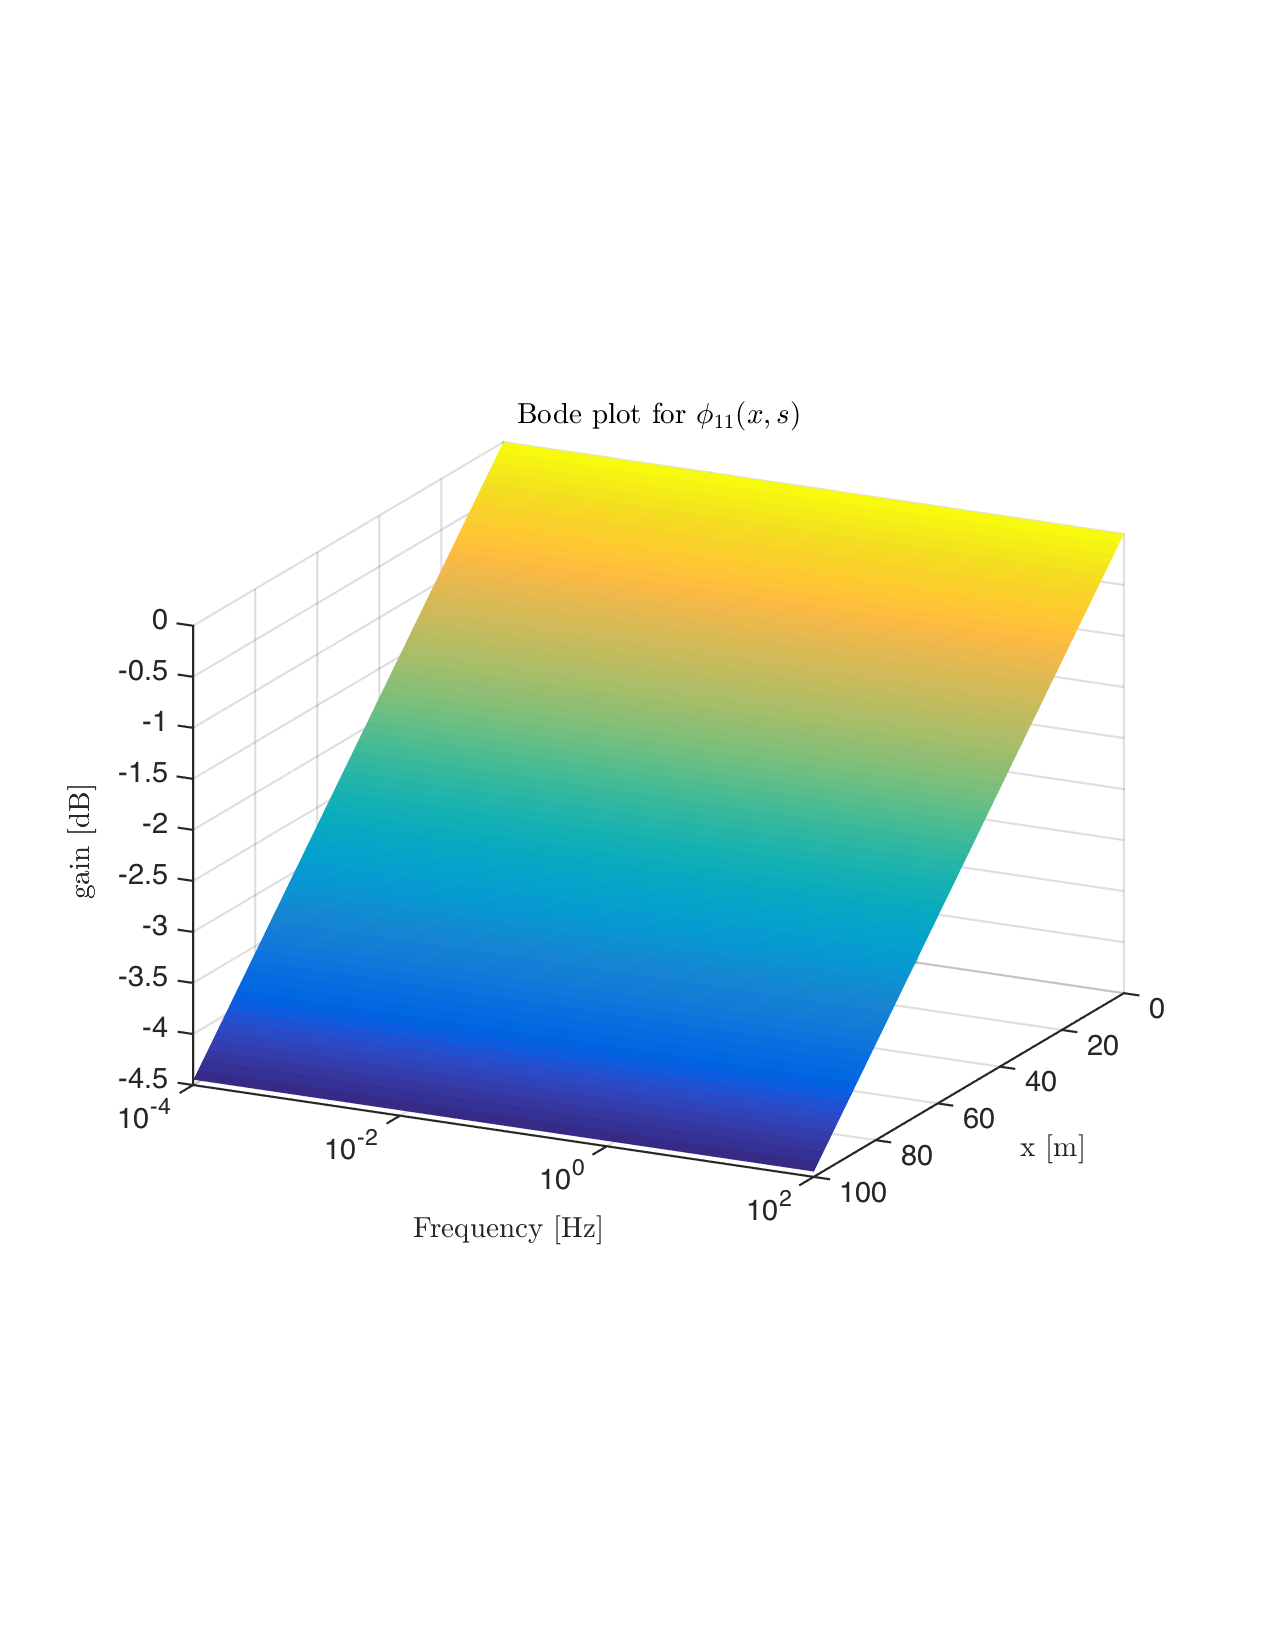
\includegraphics[trim = 0mm 60mm 0mm 60mm, width = 8cm]{distr_phi_11}
%&
%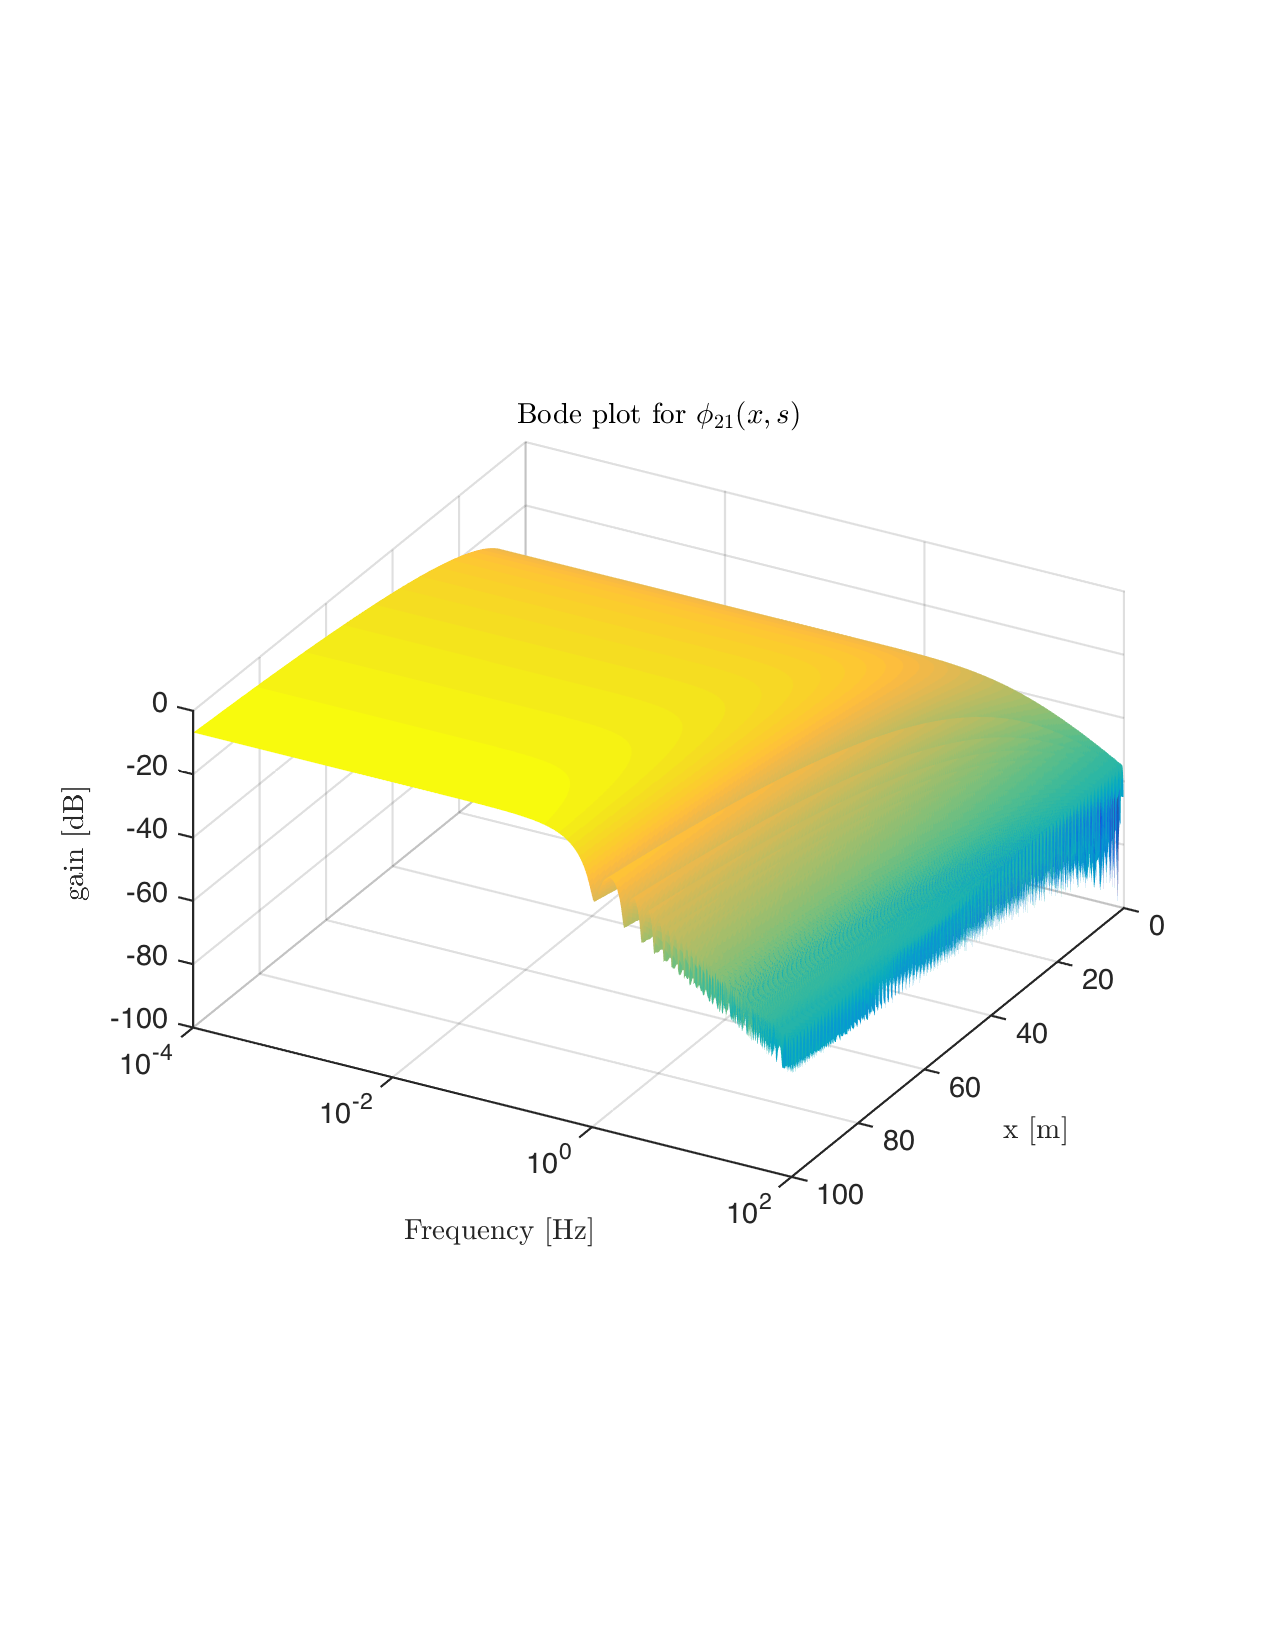
\includegraphics[trim = 0mm 60mm 0mm 60mm, width = 8cm]{distr_phi_21}
%\tabularnewline
%Spatial magnitude Bode plot for $\phi_{11}(x,s)$.
%&
%Spatial magnitude Bode plot for $\phi_{21}(x,s)$.
%\tabularnewline
%\end{tabular}
%\caption{Spatial magnitude Bode plots for Riemann invariants in free-flow regime ($\left|\alpha\right| = $ 0.53 Hz)\label{fig:Magn_spatial_diag}}
%\end{figure}
%\begin{figure}[H]
%\centering
%\includegraphics[trim = 0mm 60mm 0mm 60mm, width = 110mm]{Bode_free_flow/IO_diag}
%\caption{Magnitude and phase Bode plots for $\phi_{11}(L,s)$ and $\phi_{21}(L,s)$.\label{fig:Magn_phase_diag}}
%\end{figure}

\begin{figure}
\centering
\begin{tabular}{c}
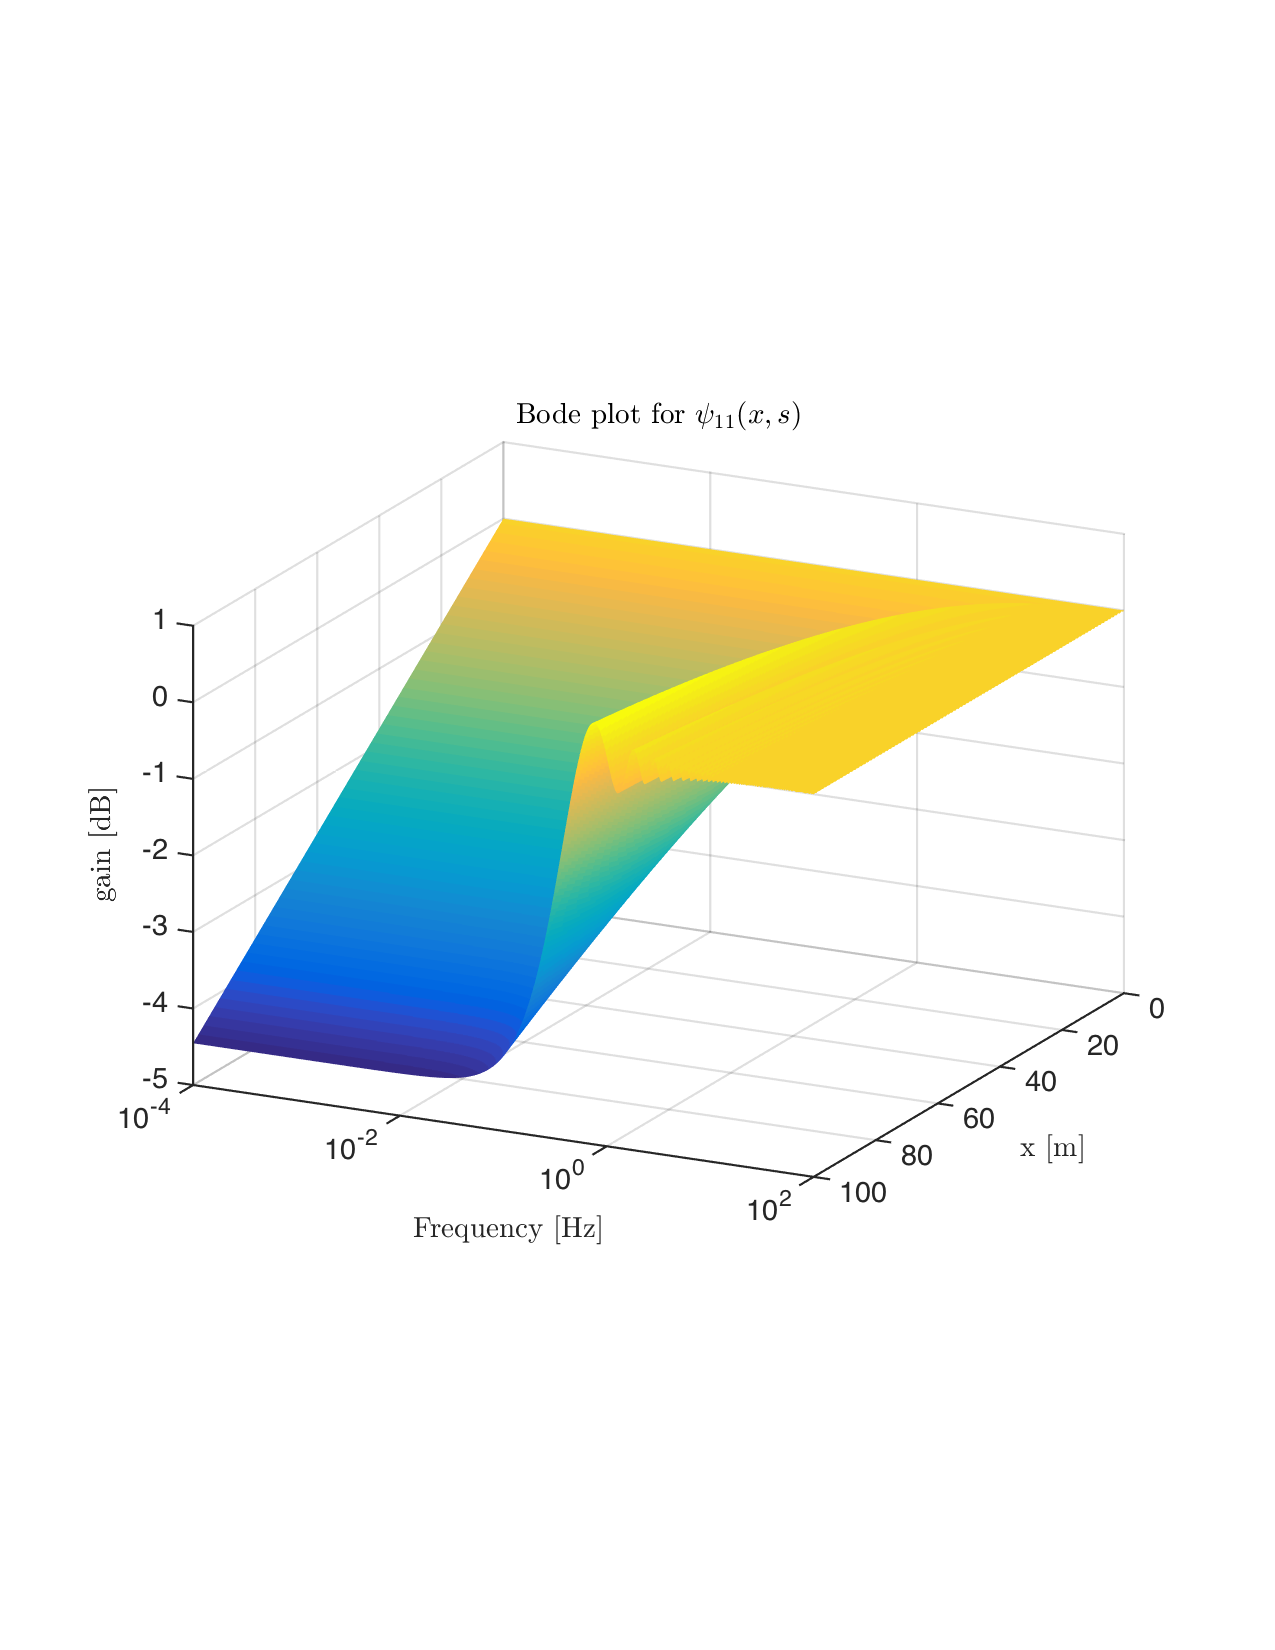
\includegraphics[trim = 0mm 60mm 0mm 60mm, width = 5cm]{distr_psi_11}
\tabularnewline
Spatial magnitude Bode plot for $\psi_{11}(x,s)$.
\tabularnewline
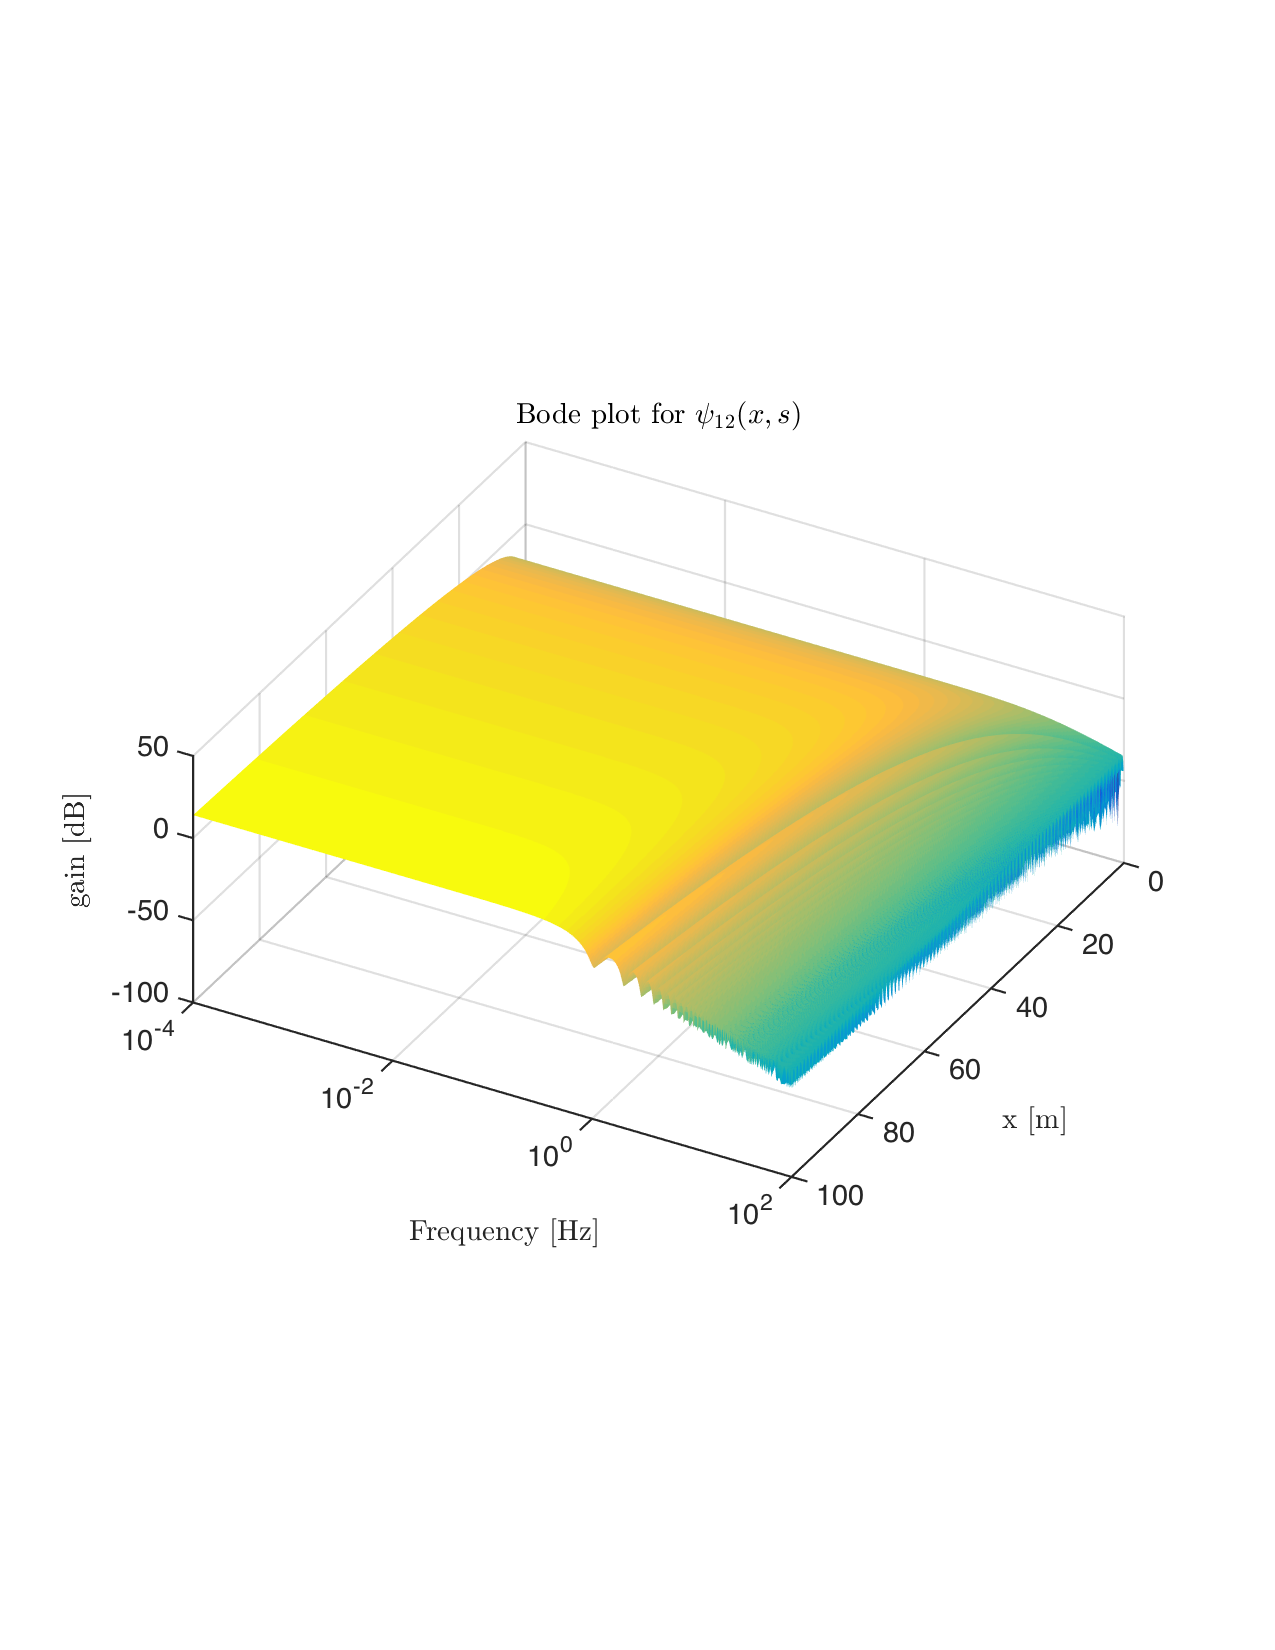
\includegraphics[trim = 0mm 60mm 0mm 60mm, width = 5cm]{distr_psi_12}
\tabularnewline
Spatial magnitude Bode plot for $\psi_{12}(x,s)$.
\tabularnewline
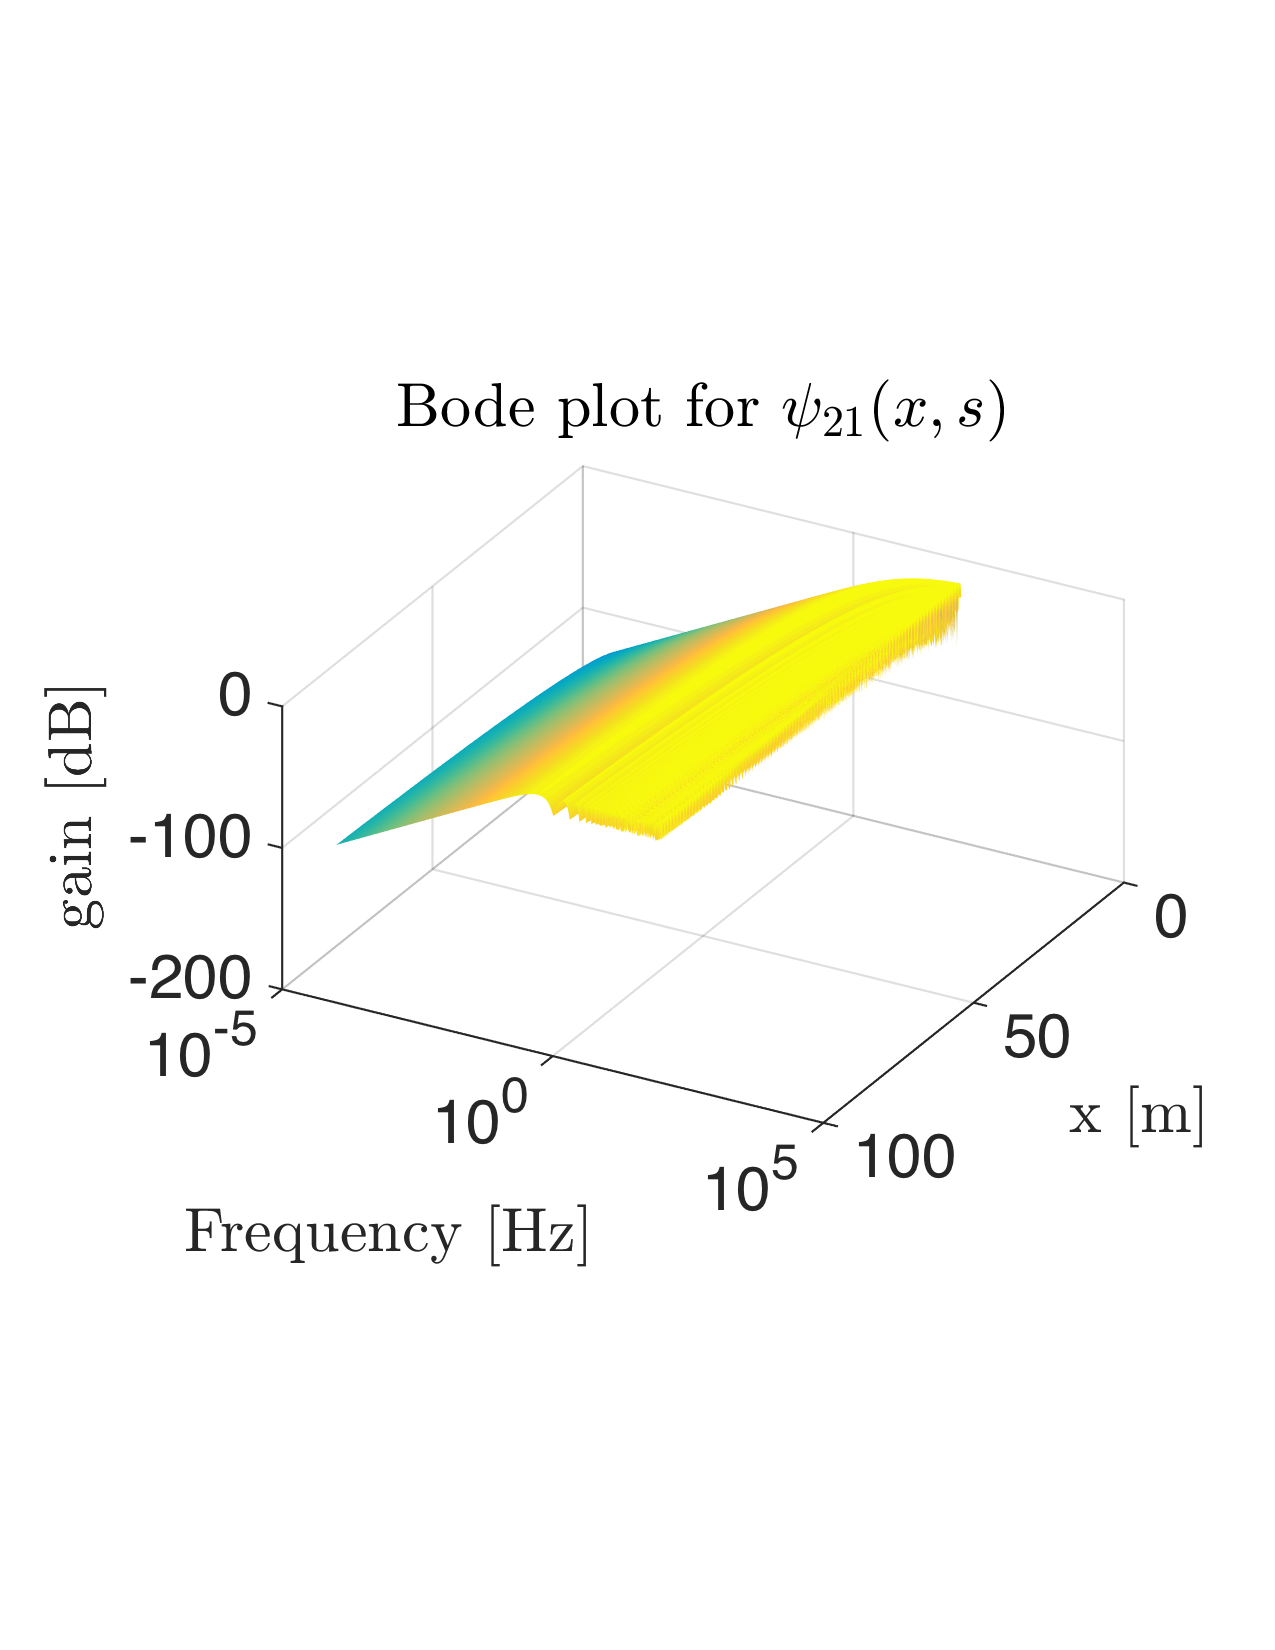
\includegraphics[trim = 0mm 60mm 0mm 60mm, width = 5cm]{distr_psi_21}
\tabularnewline
Spatial magnitude Bode plot for $\psi_{21}(x,s)$.
\tabularnewline
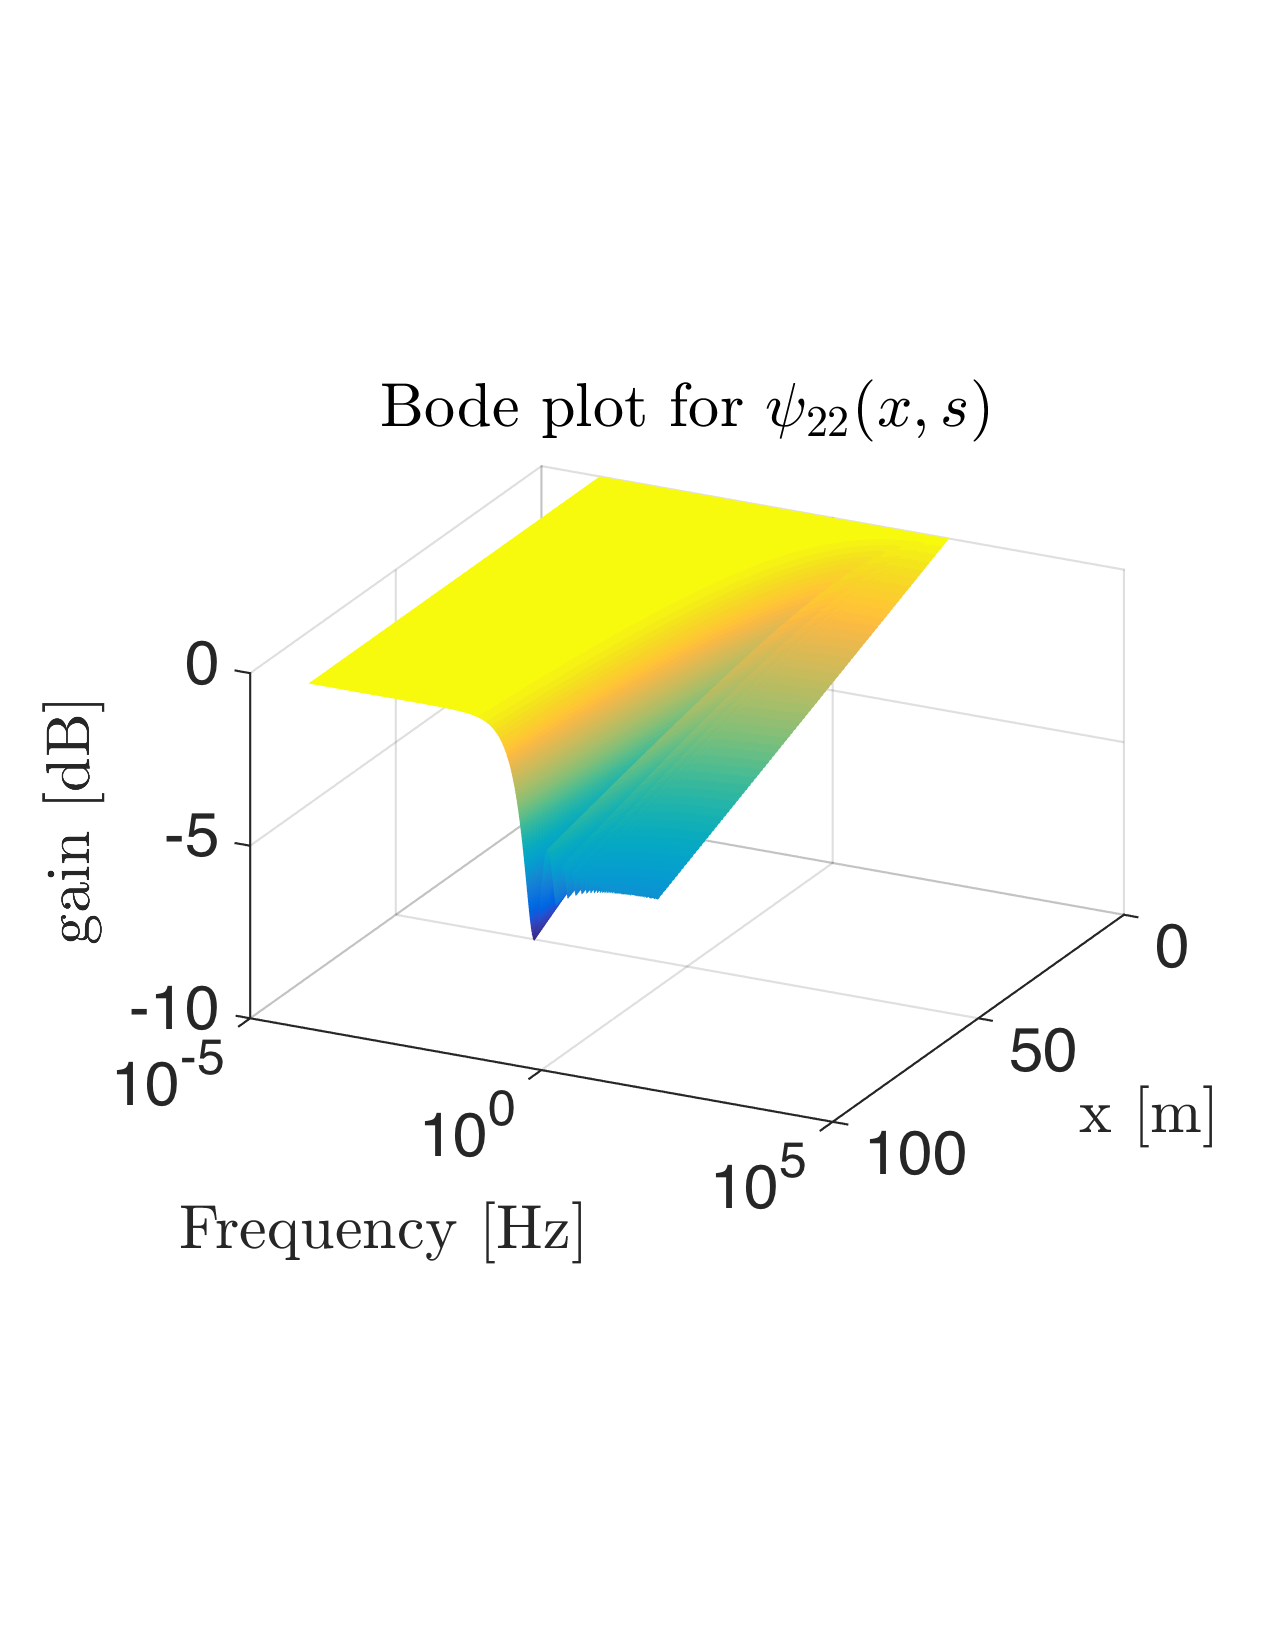
\includegraphics[trim = 0mm 60mm 0mm 60mm, width = 5cm]{distr_psi_22}
\tabularnewline
Spatial magnitude Bode plot for $\psi_{22}(x,s)$.
\end{tabular}
\caption{Spatial magnitude Bode plots for physical variables in free-flow regime ($\left|\alpha\right| = $ 0.53 Hz)\label{fig:Magn_spatial_physx}}
\end{figure}

%\begin{figure}[H]
%\centering
%\begin{tabular}{cc}
%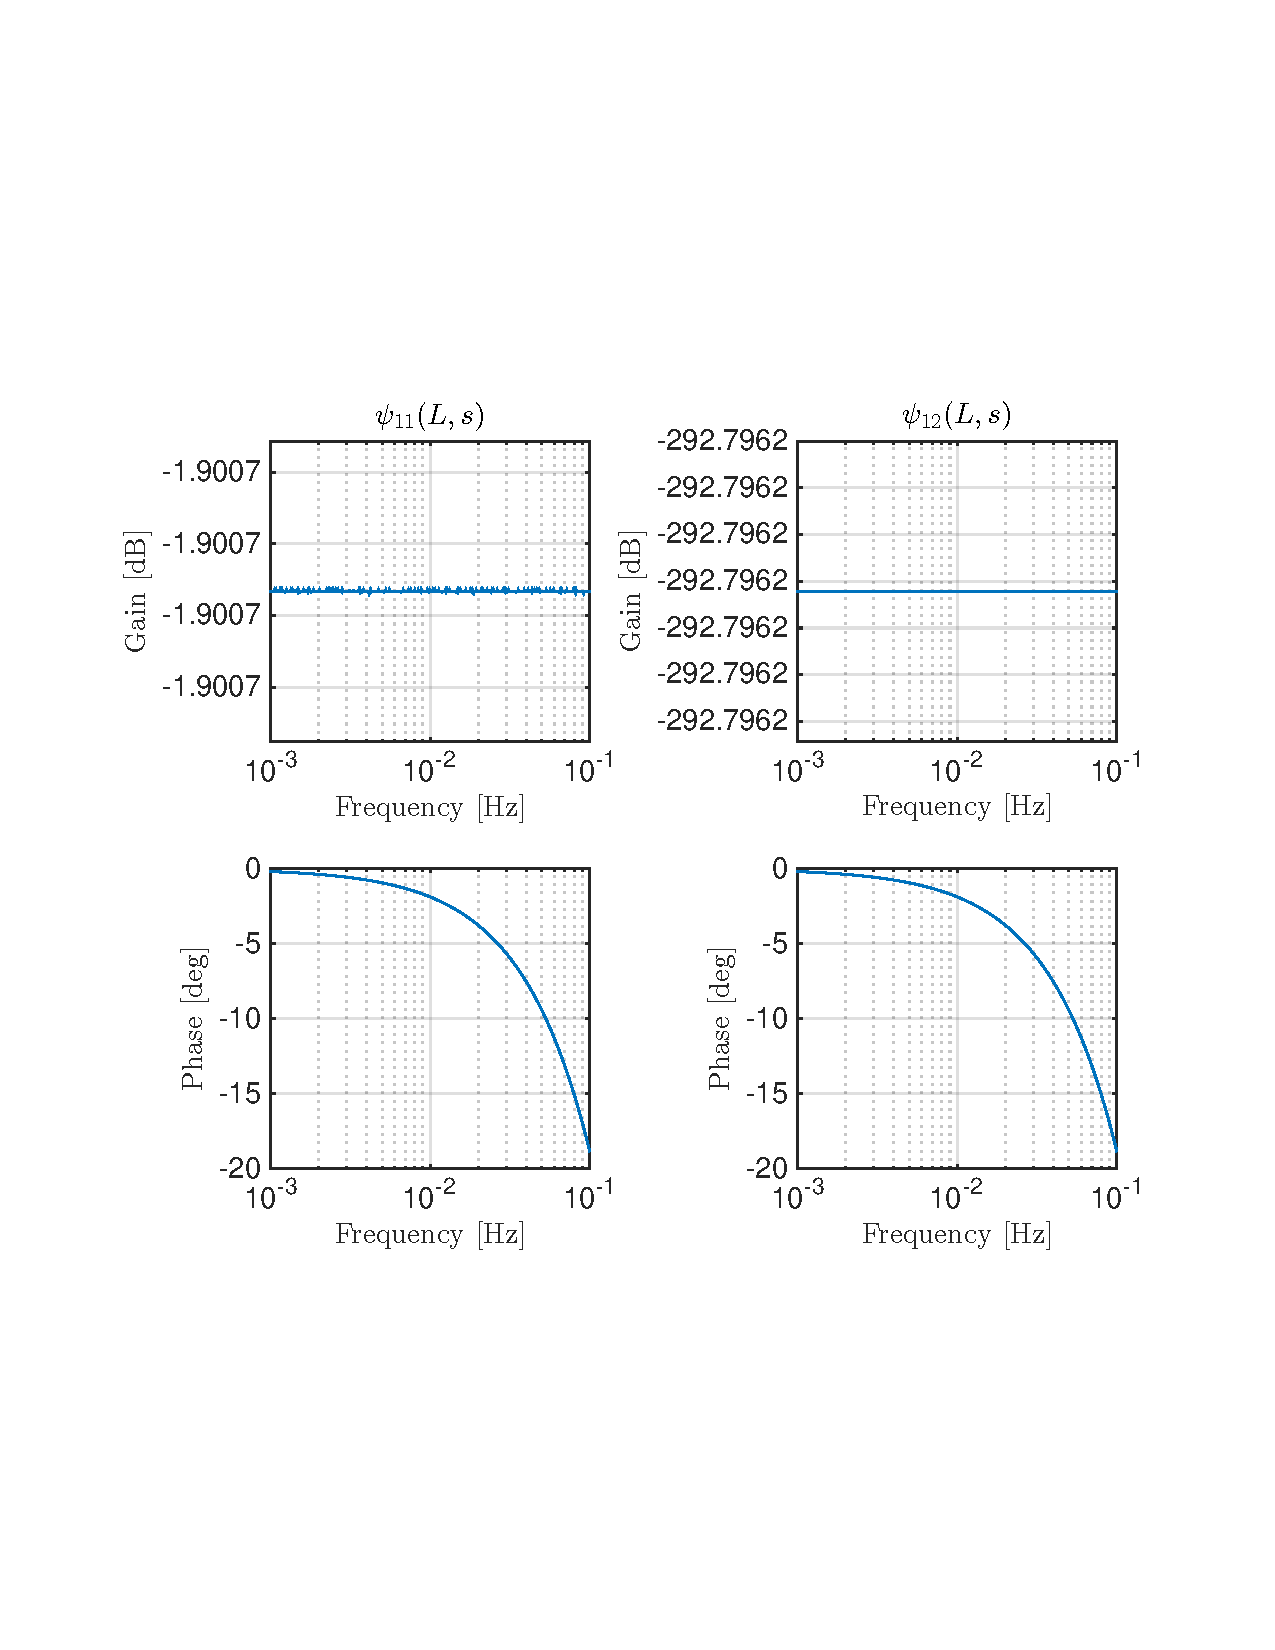
\includegraphics[trim = 0mm 60mm 0mm 60mm, width=8cm]{Bode_free_flow/IO_v}
%& 
%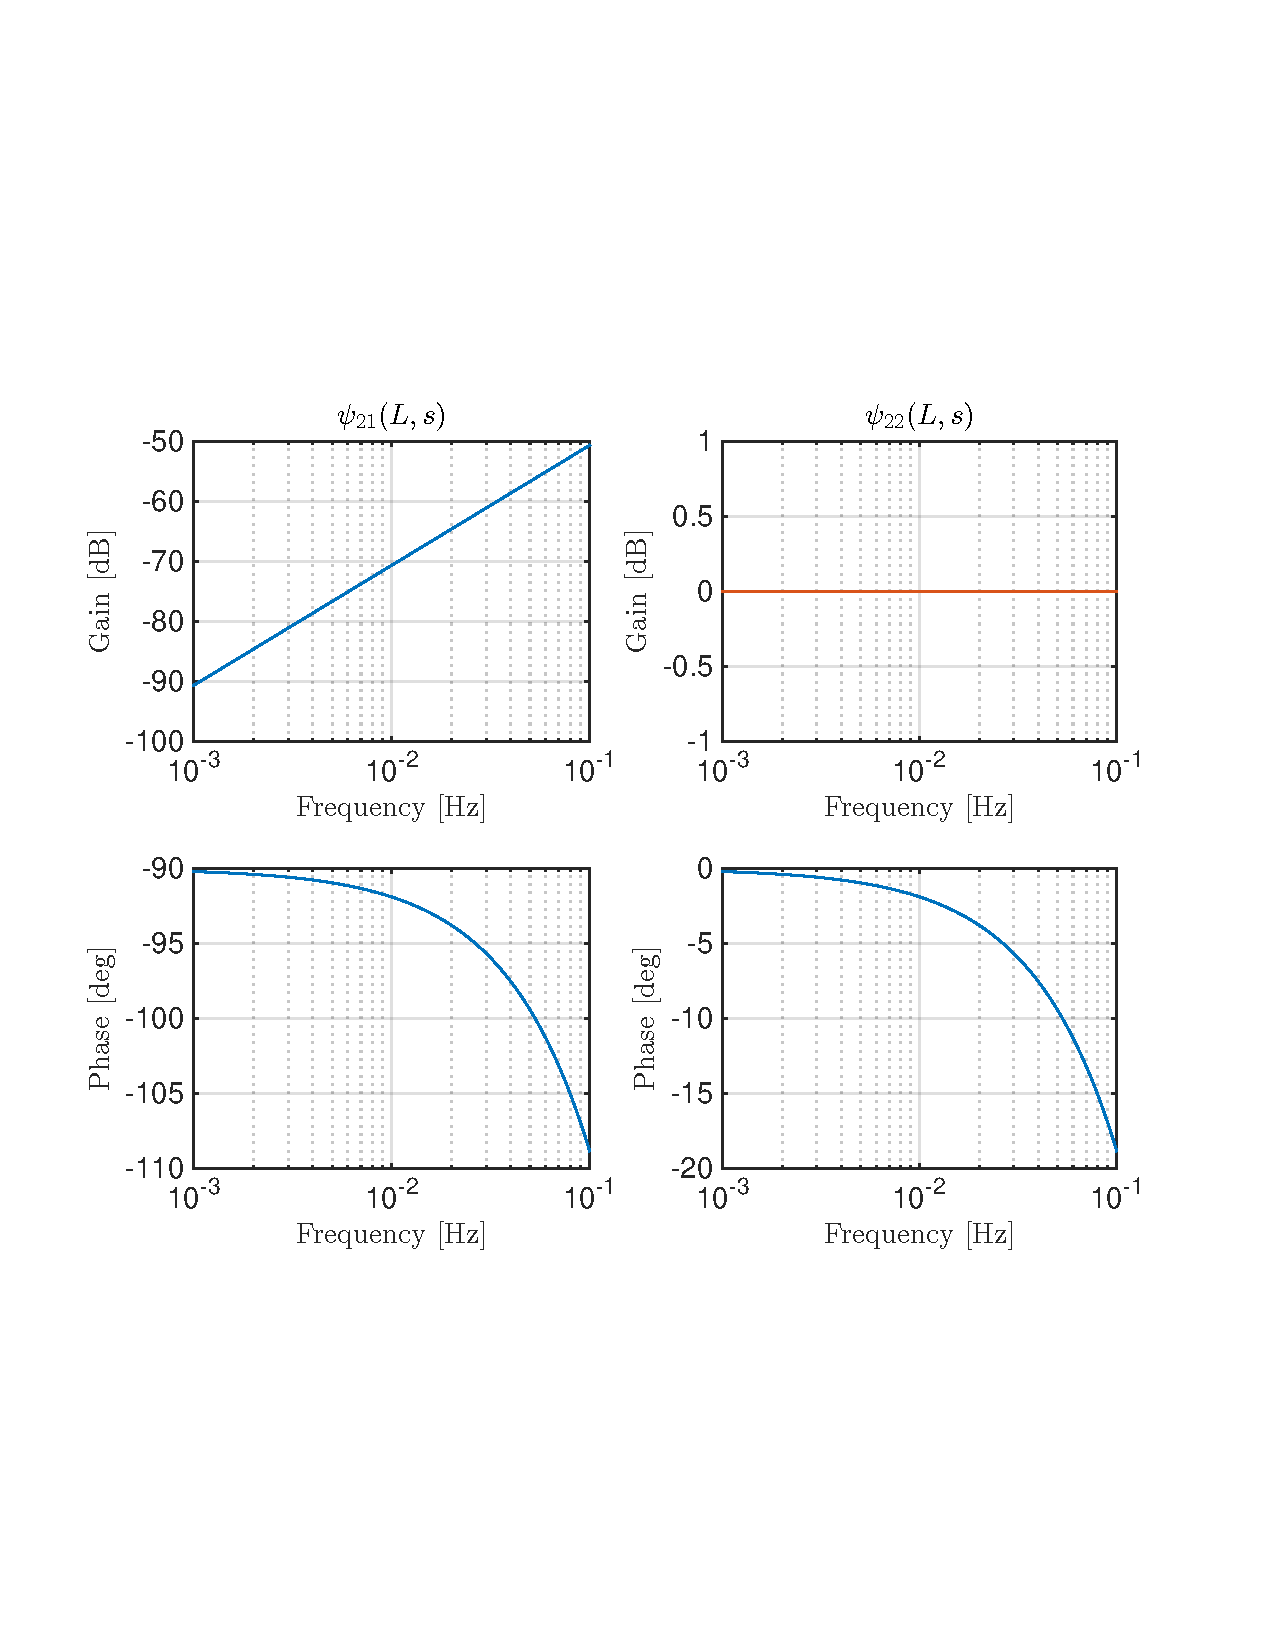
\includegraphics[trim = 0mm 60mm 0mm 60mm, width=8cm]{Bode_free_flow/IO_q}
%\tabularnewline
%\end{tabular}
%\caption{
%Magnitude and phase bode plots for $\psi_{11}(L,s)$ and $\psi_{12}(L,s)$ (left) and for $\psi_{21}(L,s)$ and $\psi_{22}(L,s)$ (right). (Physical variables).
%\label{fig:Magn_phase_physx}
%}
%\end{figure}

For transfer functions featuring $1 - e^{-\frac{x}{\lambda_{1} \tau \alpha} \left(s + \alpha \right)}$ as a factor (that is to say $\phi_{21}$, $\psi_{12}$, and $\psi_{21}$) one can observe in the corresponding Bode plots that the value of the log-gain in high frequency tends to vary very sharply. Indeed, with $s = jw$,
$
\left| 
	1 - e^{-\frac{x}{\lambda_{1} \tau \alpha} \left(s + \alpha\right)}
\right| = 
e^{-\frac{x}{\lambda_{1} \tau}}
\sqrt{
	\left(
		e^{\frac{x}{\lambda_{1}\tau}} 
		-
		\cos\left(\frac{w}{\lambda_{1} \tau \alpha} x\right)
	\right)^{2}
	+
	\sin^{2}\left( \frac{w}{\lambda_{1} \tau \alpha} x \right)
}
$. Therefore, if the spatial pseudo-period $\tilde{L}=\frac{2\pi}{w} \lambda_{1} \tau \left|\alpha\right|$ is low enough, near zero values appear when $x$ is a multiple of $\tilde{L}$. This explains the irregular shape of the distributed Bode plots of $\phi_{21}$, $\psi_{12}$, and $\psi_{21}$ for frequencies $w \gg 2 \pi \frac{\lambda_{1} \tau \left|\alpha\right|}{L} = 6.53$ Hz. This does not impact the stability of the system. Bode plots only look irregular about such points because of the logarithmic scale.

\subsubsection{Step responses}
We analyze the behavior of the system given step inputs $\tilde{v}(0,t)=\bar{v}H(t)$ and $\tilde{q}(0,t)=\bar{q}H(t)$, where $H(\cdot)$ is the Heaviside function. The step responses can be explicitly computed from the spectral responses, let $H_1(t,x) = H\left(t-\frac{x}{\lambda_{1}}\right)$ and
$H_2(t,x) = H\left(t - \frac{x}{\lambda_{2}} \right)$:

\begin{align} 
\tilde{v}(x,t) &= 
\bar{v}
e^{-\frac{x}{\lambda_{1}\tau}}H_1(t,x)
\notag\\
&\quad
+\bar{v}
e^{-\alpha \left(t - \frac{x}{\lambda_{2}} \right)}
	(H_2 - H_1)(t,x)
\notag \\
&\quad
- \dfrac{\bar{q}}{\rho^* \tau}
\left(
	e^{-\frac{x}{\lambda_{1}\tau}}H_1\left(t,x\right) 
	- H_2(t,x)
\right) 
\notag\\
&\quad
- \dfrac{\bar{q}}{\rho^* \tau} e^{-\alpha \left(t - \frac{x}{\lambda_{2}} \right)}
	(H_2 - H_1)(t,x)\\
\tilde{q}(x,t) &= \bar{v} \rho^*\tau \alpha e^{-\alpha \left(t - \frac{x}{\lambda_{2}} \right)}
	(H_1 - H_2)(t,x)
\notag \\
&\quad+ 
\bar{q}
H_2(t,x)
\notag\\
&\quad
+
\bar{q}
e^{-\alpha \left(t - \frac{x}{\lambda_{2}} \right)}
	(H_1 - H_2)(t,x)	
\end{align}

With this set of time domain expressions, we can see that a cone of exponentially growing speed and flow linearization errors generally appears between the characteristic lines corresponding to $\lambda_{1}$ and $\lambda_{2}$. This is caused by $\alpha$ being negative in the free flow regime and means that, in this region of the domain $\left[0,T\right] \times \left[0,L\right]$, the $\left(v,q\right)$ state of the linearized system can diverge exponentially fast from the linearization point. This is consistent with the observations in \cite{PhysRevLett.79.4030} where small local perturbations occurring in free-flow regime can cause traffic to transition durably to the congested regime.

\begin{figure}
\begin{centering}
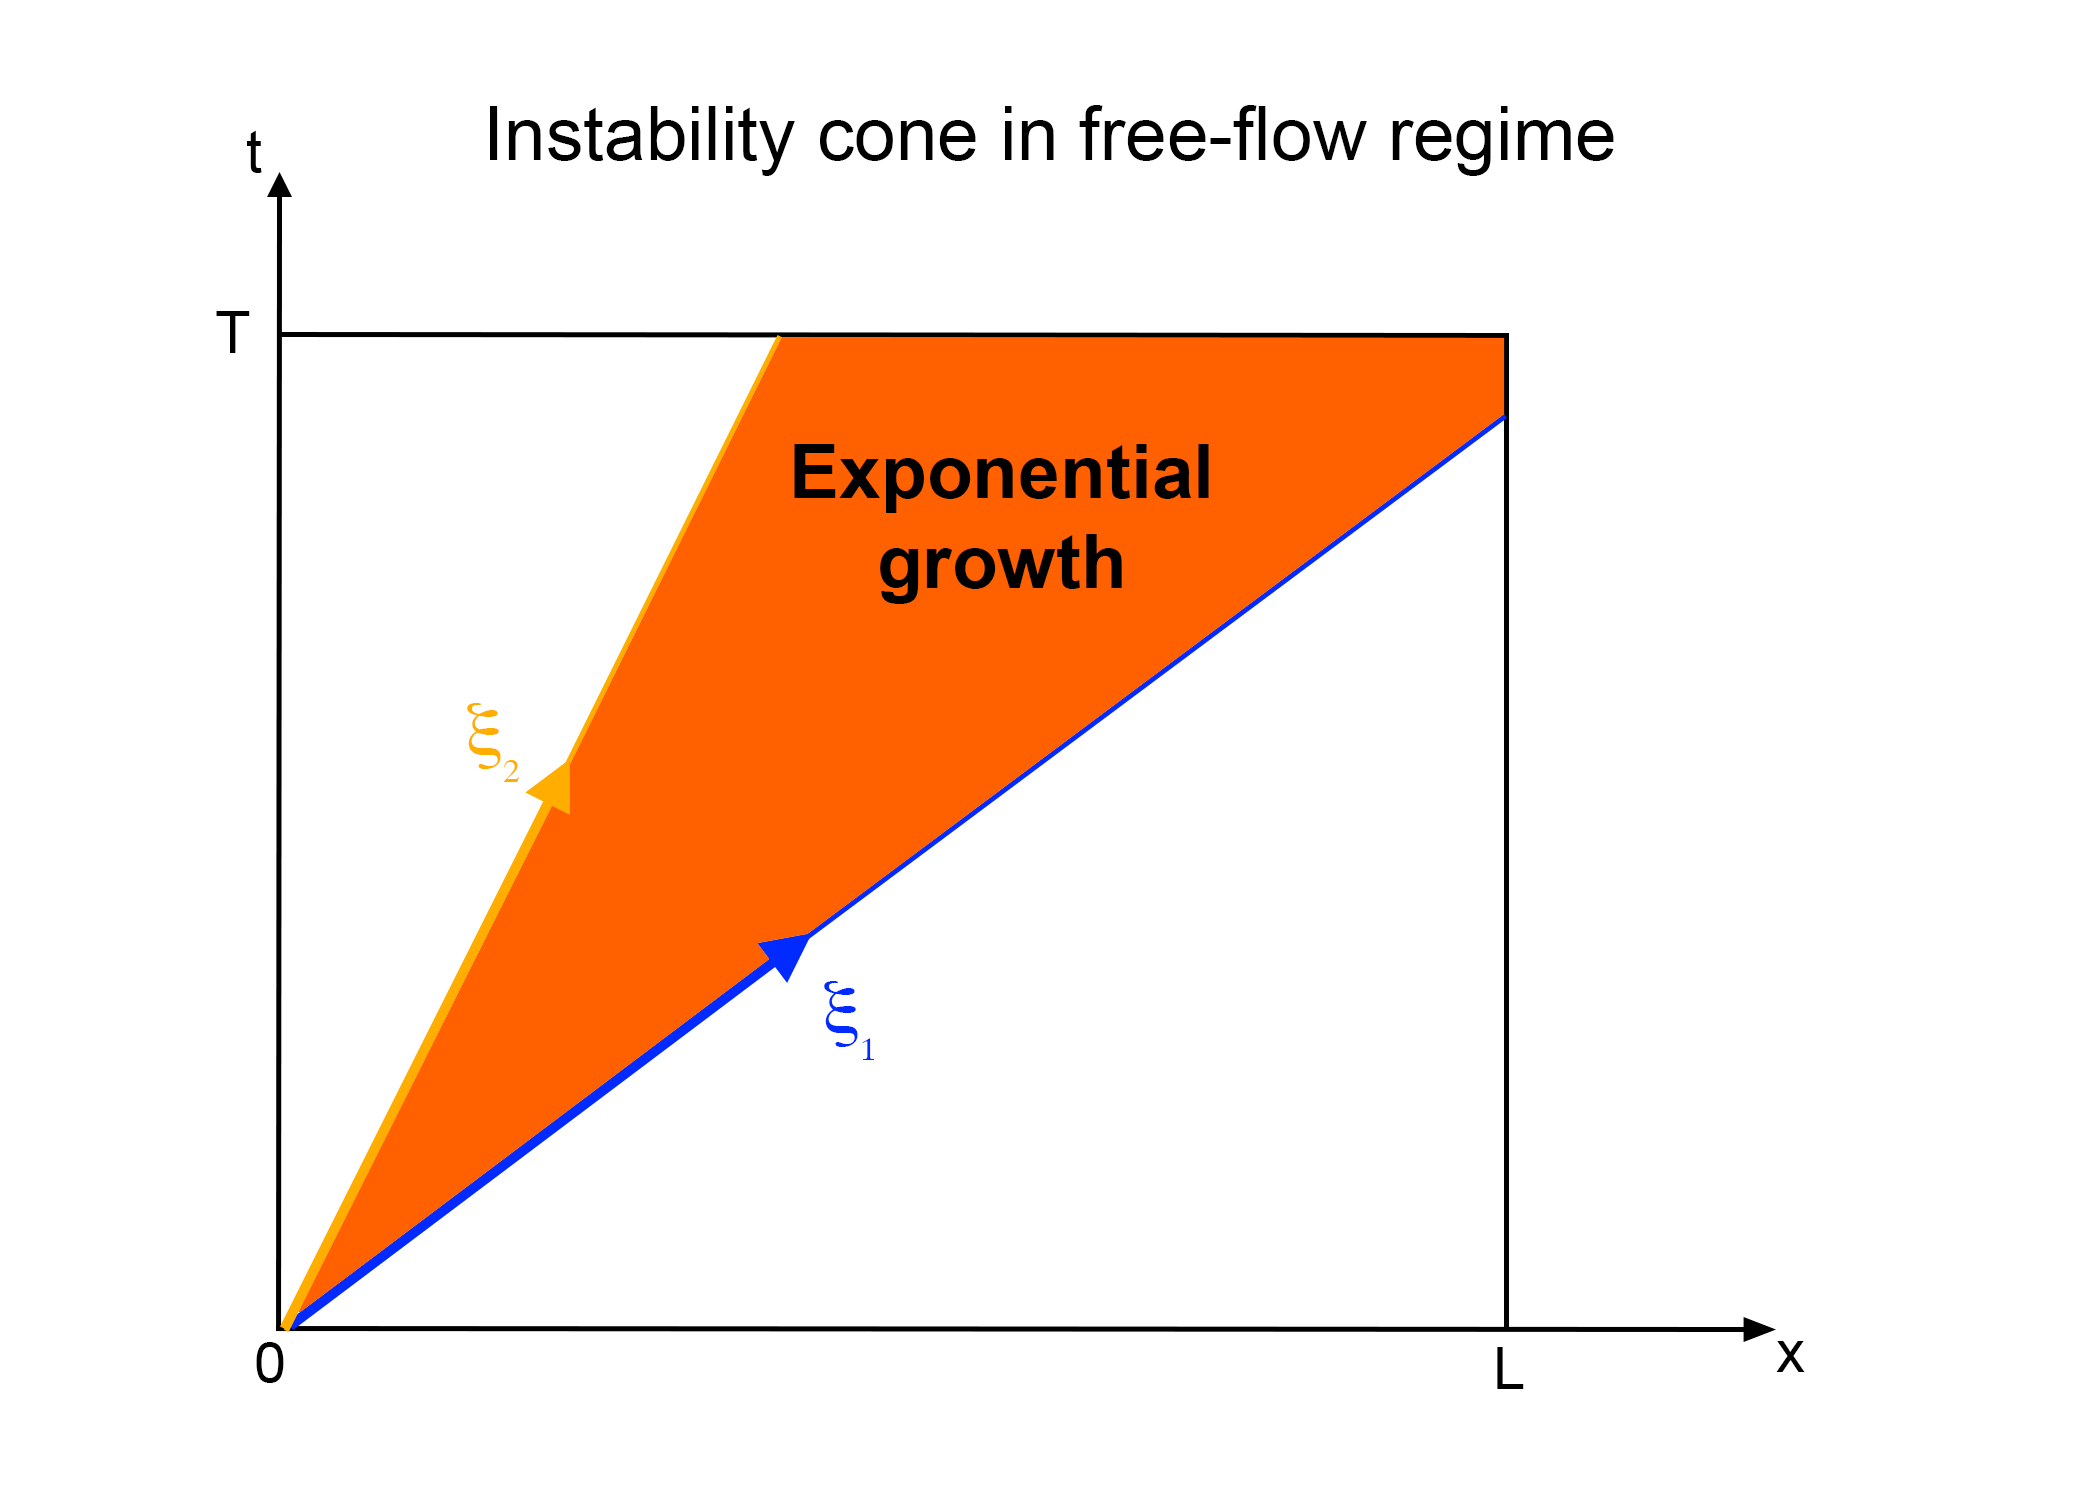
\includegraphics[width=6cm]{Exp-growth}
\par\end{centering}
\protect\caption{Illustration of the exponential growth cone appearing in the free-flowing regime for the time domain expressions of $v$ and $q$.\label{Exp-growth}}
\end{figure}

\subsection{Congested regime ($F>1$)}
We now consider the system in the congested regime.

Using \eqref{TFRiemann} we can write 
\begin{equation} \label{vqcongested}
\begin{pmatrix}
	\hat{\xi_{1}}(x,s)\\
	\hat{\xi_{2}}(x,s)
\end{pmatrix} = 
\Gamma(x,s)
\begin{pmatrix}
	\hat{\xi_{1}}\left(0,s\right)\\
	\hat{\xi_{2}}\left(L,s\right)
\end{pmatrix}.
\end{equation}
with 
\begin{subequations}
\begin{align}
\gamma_{11}\left(x,s\right)&=
e^{-\frac{x}{\lambda_{1}}\left(s+\frac{1}{\tau}\right)} , \\
\gamma_{12}\left(x,s\right)&=0, \\
\gamma_{21}\left(x,s\right)&=
\frac{\lambda_{1} \alpha e^{-\frac{x}{\lambda_{1}} \left( s + \frac{1}{\tau} \right)}}
{\lambda_{2}\left(s + \alpha\right)}
\left(
	1 -
	e^{-\frac{\left(L - x\right)
		}{
		\lambda_{1}\tau\alpha
		}
		\left(s+\alpha\right)
		}
\right)
, \\
\gamma_{22}\left(x,s\right)&=e^{\frac{s\left(L-x\right)}{\lambda_{2}}}.
\end{align}
\end{subequations}

Note that equation \eqref{vqcongested} corresponds to a closed form solution of our initial system, written in spectral form.

For low frequencies ($\left|s\right|\ll\left|\alpha\right|$), 
$\gamma_{21}\left(x,s\right)
\simeq
\frac{\lambda_{1}}{\lambda_{2}}
e^{-\frac{x}{\lambda_{1}} \left( s + \frac{1}{\tau} \right)}
\left(
	1 -
	e^{-\frac{L-x}{\lambda_{1}\tau}}
\right)
$
is the combination of a gain, a distributed delay with propagation speed $\lambda_{1}$, and two distributed gains with characteristic distance $\lambda_{1}\tau$ that cancel out for $x = L$. The resulting bode plot is presented below in Figure \ref{fig:Magn_spatial_diag_congested}.

\subsubsection{Transfer functions for physical variables in congested regime}
In congested regime, the boundary conditions used to control the system are $\hat{\xi}_{1}\left(0,\cdot\right)$ and $\hat{\xi}_{2}\left(0,\cdot\right)$. By linearity of the Laplace transform 
$\hat{\xi_{1}}\left(0,s\right) = 
\frac{
	\rho^{*}\lambda_{2}
}{
	\lambda_{1} - \lambda_{2}
} 
\hat{v}\left(0,s\right)
+
\hat{q}\left(0,s\right)
$.
Therefore, as
$\hat{\xi_{2}}\left(0,s\right) =
\gamma_{21}\left(0,s\right)
\hat{\xi_{1}}\left(0,s\right)
+
\gamma_{22}\left(0,s\right)
\hat{\xi_{2}}\left(L,s\right)$
, we get
$\hat{\xi_{1}}\left(0,s\right) =
\frac{1}{d\left(s\right)}
\hat{q}\left(0,s\right)
+
\frac{n\left(s\right)}{d\left(s\right)}
\hat{v}\left(L,s\right)
$
where
$d\left(s\right) = 1 - \frac{\lambda_{2}}{\lambda_{1}}\gamma_{21}\left(0,s\right)$
and
$n\left(s\right) = \frac{\rho^{*} \lambda_{2}}{\lambda_{1} - \lambda_{2}} \gamma_{22}\left(0,s\right)$. The $\left(v,q\right)$ system has only two degrees of freedom. Therefore we consider that the only inputs to the system are $q\left(0,\cdot\right)$ and $v\left(L,\cdot\right)$. $v\left(0,\cdot\right)$ is then completely determined and can be interpreted as an output of the system. The corresponding transfer equation is
\begin{equation}
\begin{pmatrix}
	\hat{v}\left(x,s\right)
	\\
	\hat{q}\left(x,s\right)
\end{pmatrix}
=
\underset{\Theta\left(x,s\right)}{
\underbrace{
R^{-1}\Gamma\left(x,s\right)
\begin{pmatrix}
	\frac{n\left(s\right)}{d\left(s\right)}
		&
	\frac{1}{d\left(s\right)}	
	\\
	\frac{\rho^{*}\lambda_{1}}{\lambda_{1} - \lambda_{2}}
		&
	0
\end{pmatrix}
}
}
\begin{pmatrix}
	\hat{v}\left(L,s\right)
	\\
	\hat{q}\left(0,s\right)
\end{pmatrix}
\end{equation}
where
\begin{subequations}
\begin{align}
\theta_{11}\left(x,s\right) &=
\frac{
	\alpha 
		e^{
			-\frac{x}{\tau\lambda_{1}}
		}
		e^{
			-\frac{s}{\lambda_{1}}
				\left(
					x - L\frac{\lambda_{1}}{\lambda_{2}}
				\right)	
		}
	+
	s 
		e^{-\frac{s}{\lambda_{2}}\left(x - L\right)}
}{
	s
	+
	\alpha
	e^{-\frac{L}{\tau\lambda_{1}}}
	e^{
	-\frac{sL}{\lambda_{1}}
	\left(
		1 - \frac{\lambda_{1}}{\lambda_{2}}
	\right)
	}
}
,\\
\theta_{12}\left(x,s\right) &=
\frac{
	e^{-\frac{L}{\tau\lambda_{1}}}
	e^{-\frac{s}{\lambda_{2}}
		\left(
			x - L
				\left(1 - 
					\frac{\lambda_{2}}{\lambda_{1}}
				\right)
		\right)
	}
	-
	e^{-\frac{x}{\tau\lambda_{1}}}
	e^{-\frac{sx}{\lambda_{1}}}
}
{
	\rho^{*}\tau
	\left(
		s
		+
		\alpha
		e^{-\frac{L}{\tau\lambda_{1}}}
		e^{
			-\frac{sL}{\lambda_{1}}
			\left(
				1 - \frac{\lambda_{1}}{\lambda_{2}}
			\right)
			}
	\right)
},\\
\theta_{21}\left(x,s\right) &=
\rho^{*}\tau\alpha s
\frac{
	e^{-\frac{s\left(x-L\right)}{\lambda_{2}}}
	-
	e^{-\frac{x}{\tau\lambda_{1}}}
	e^{-\frac{s}{\lambda_{1}}
		\left(
			x - L\frac{\lambda_{1}}{\lambda_{2}}
		\right)
	}
}{
	s
	+
	\alpha
	e^{-\frac{L}{\tau\lambda_{1}}}
	e^{
	-\frac{sL}{\lambda_{1}}
	\left(
		1 - \frac{\lambda_{1}}{\lambda_{2}}
	\right)
	}
},\\
\theta_{22}\left(x,s\right) &=
\frac{
	\alpha
	e^{-\frac{L}{\tau\lambda_{1}}}
	e^{-\frac{s}{\lambda_{2}}
		\left(
			x - L
				\left(
				1 - \frac{\lambda_{2}}{\lambda_{1}}
				\right)
		\right)
	}
	+
	s
	e^{-\frac{x}{\tau\lambda_{1}}}
	e^{-\frac{sx}{\lambda_{1}}}
}{
	s
	+
	\alpha
	e^{-\frac{L}{\tau\lambda_{1}}}
	e^{
	-\frac{sL}{\lambda_{1}}
	\left(
		1 - \frac{\lambda_{1}}{\lambda_{2}}
	\right)
	}
}
.
\end{align}
\end{subequations}

\subsubsection{Low frequency approximation for physical variables in congested regime}
We derive approximate expressions in the frequency domain for the transfer functions above when $\left|s\right|\ll\left|\alpha\right|$:
\begin{subequations}
\begin{align}
\theta_{11}\left(x,s\right) &\simeq
e^{\frac{s\left(L-x\right)}{\lambda_{2}}}
e^{\frac{L-x}{\tau\lambda_{1}}},\\
\theta_{12}\left(x,s\right) &\simeq
\frac{1}{\rho^{*}\tau\alpha}
e^{-\frac{sx}{\lambda_{1}}}
\left(
	1 - e^{\frac{L-x}{\tau\lambda_{1}}}
\right),\\
\theta_{21}\left(x,s\right) &\simeq
s \rho^{*}\tau
e^{\frac{s\left(L-x\right)}{\lambda_{2}}}
e^{\frac{L}{\tau\lambda_{1}}}
\left(
	1 - e^{-\frac{x}{\tau\lambda_{1}}}
\right),\\
\theta_{22}\left(x,s\right) &\simeq
e^{-\frac{sx}{\lambda_{1}}}.
\end{align}
\end{subequations}

With such expressions, interpreting the approximate transfer functions in low frequencies becomes fairly easy:
\begin{itemize}
\item The transfer function $\theta_{11}$ (resp. $\theta_{12}$) appears as the combination of a distributed delay with propagation speed $-\lambda_{2}$ (resp. $\lambda_{1}$) and a distributed gain (resp. attenuation) with characteristic distance $\lambda_{1}\tau$.
\item The structure of $\theta_{21}$ is similar to that of $\theta_{11}$ although it features a derivator component.
\item Once simplified, $\theta_{22}$ corresponds to a distributed delay with propagation speed $\lambda_{1}$.
\item Hypothetical poles are not active in the range of low frequencies that will be considered in our traffic flow modeling applications.
\end{itemize}

%Comparing the approximate expressions of the transfer functions for $v$ and $q$ in free-flow ($\Psi\left(x,s\right)$) and congested regime ($\Theta\left(x,s\right)$) also highlights their being extremely similar. For the them to match perfectly it is necessary to replace $x$ by $L-x$ in some gain and delay elements. These changes relate to the fact that in free-flow regime both boundary conditions for $\hat{v}$ and $\hat{q}$ were defined at $x=0$ whereas in congested regime $\hat{v}$ is set at $x=L$ and $\hat{q}$ at $x=0$.

\subsubsection{Bode plots for congested regime}
We use the same fundamental diagram as in the free-flow case. However the linearization point, $\rho^* = 0.08$ veh/m, corresponds to the congested region of the Greeshields diagram. We show the distributed Bode plots for the Riemann invariants in Figure \ref{fig:Magn_spatial_diag_congested} and for the physical variables in Figure . In that case, $\alpha =$ 0.05 Hz, which does correspond to a reasonable characteristic frequency for traffic modeling applications.

Similarly to the free-flow case, for high frequencies ($w \gg 2 \pi \frac{\lambda_{1} \tau \alpha}{L} = 0.13$ Hz) near zero values appearing with spatial periodicity $\frac{2 \pi}{w} \lambda_{1} \tau \alpha$ almost cancel out $\gamma_{21}$, $\theta_{12}$, and $\theta_{21}$. Such points only appear as irregularities in the Bode plots because the gain is computed on a logarithmic scale.

%\begin{figure}[H]
%\centering
%\includegraphics[trim = 0mm 60mm 0mm 60mm, width=8cm]{Bode_congested/IO_diag}
%\caption{
%Magnitude and phase bode plots for $\gamma_{11}(L,s)$ and $\gamma_{21}(L,s)$ (left). (Riemann invariants).
%\label{fig:Magn_phase_physx_congested}
%}
%\end{figure}

%\begin{figure}
%\centering
%\begin{tabular}{cc}
%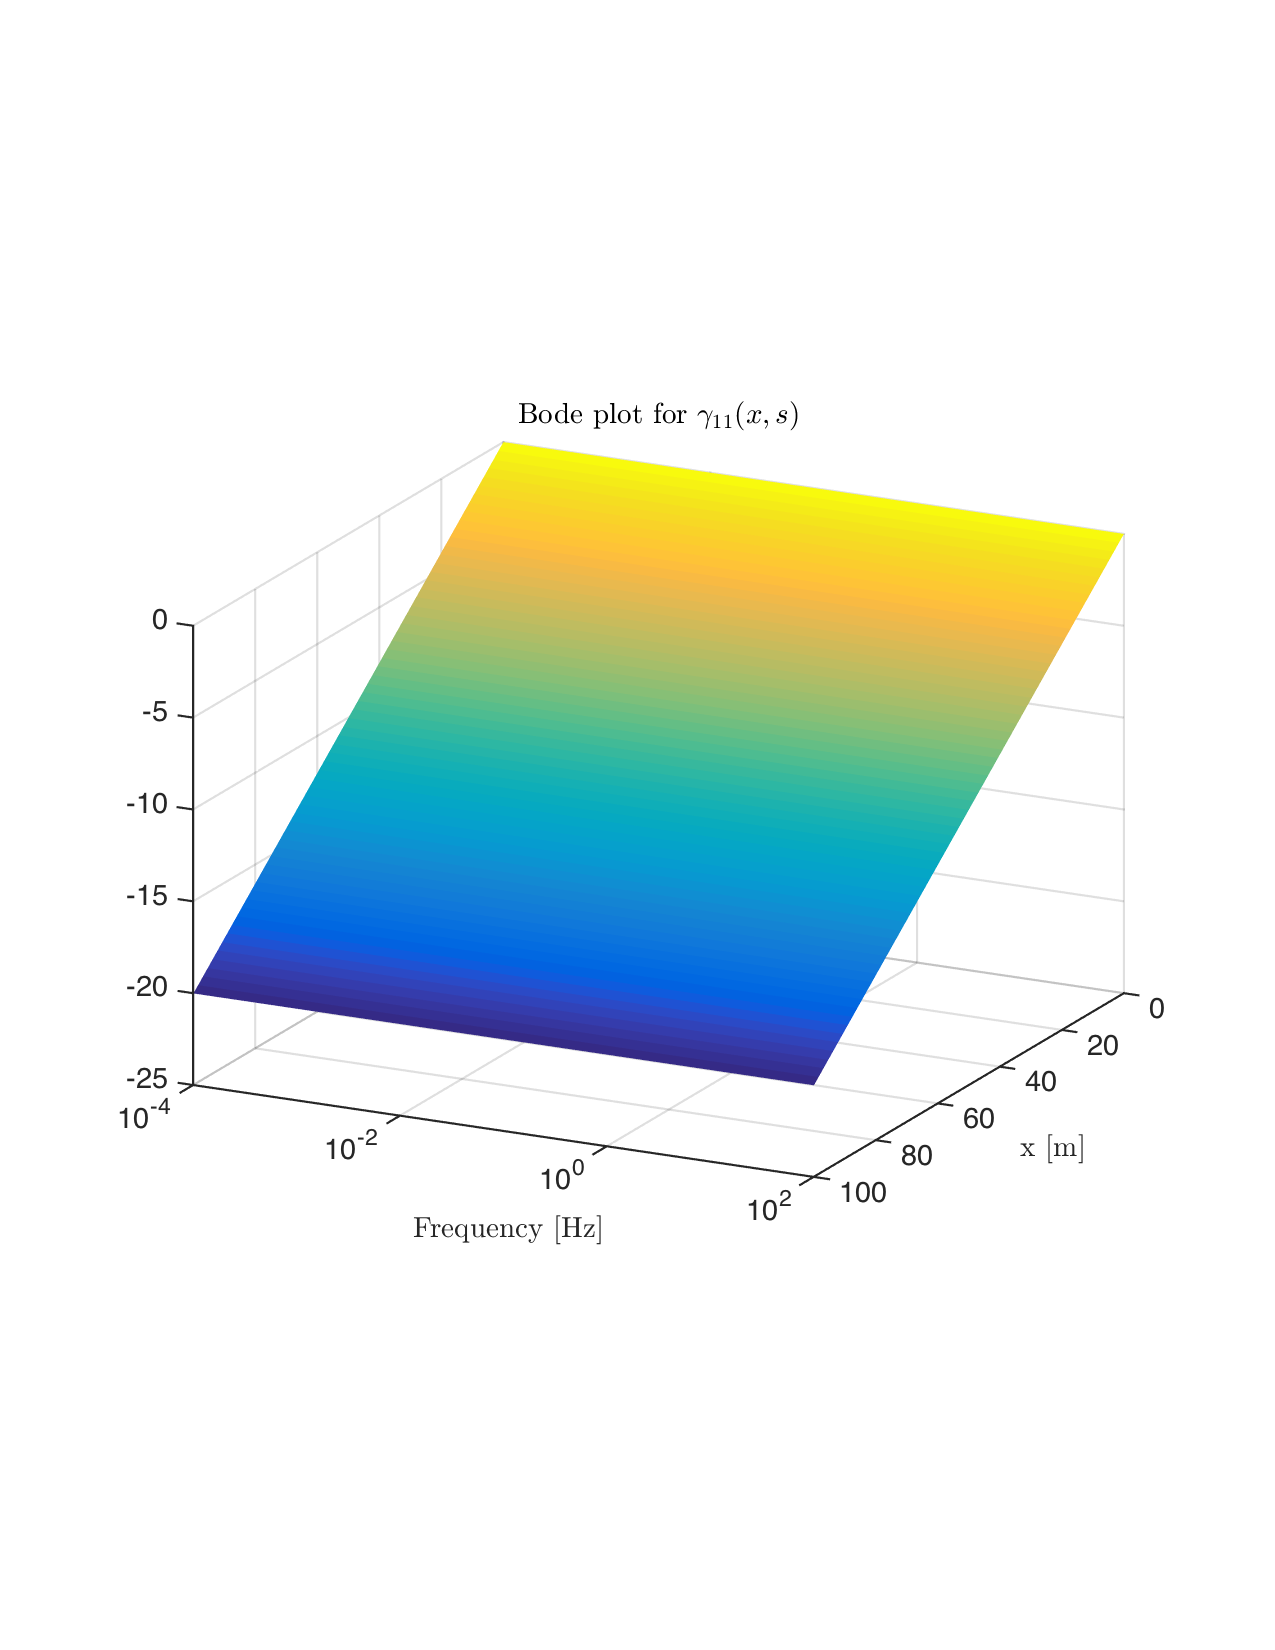
\includegraphics[trim = 0mm 60mm 0mm 60mm, width = 8cm]{distr_gamma_11}
%&
%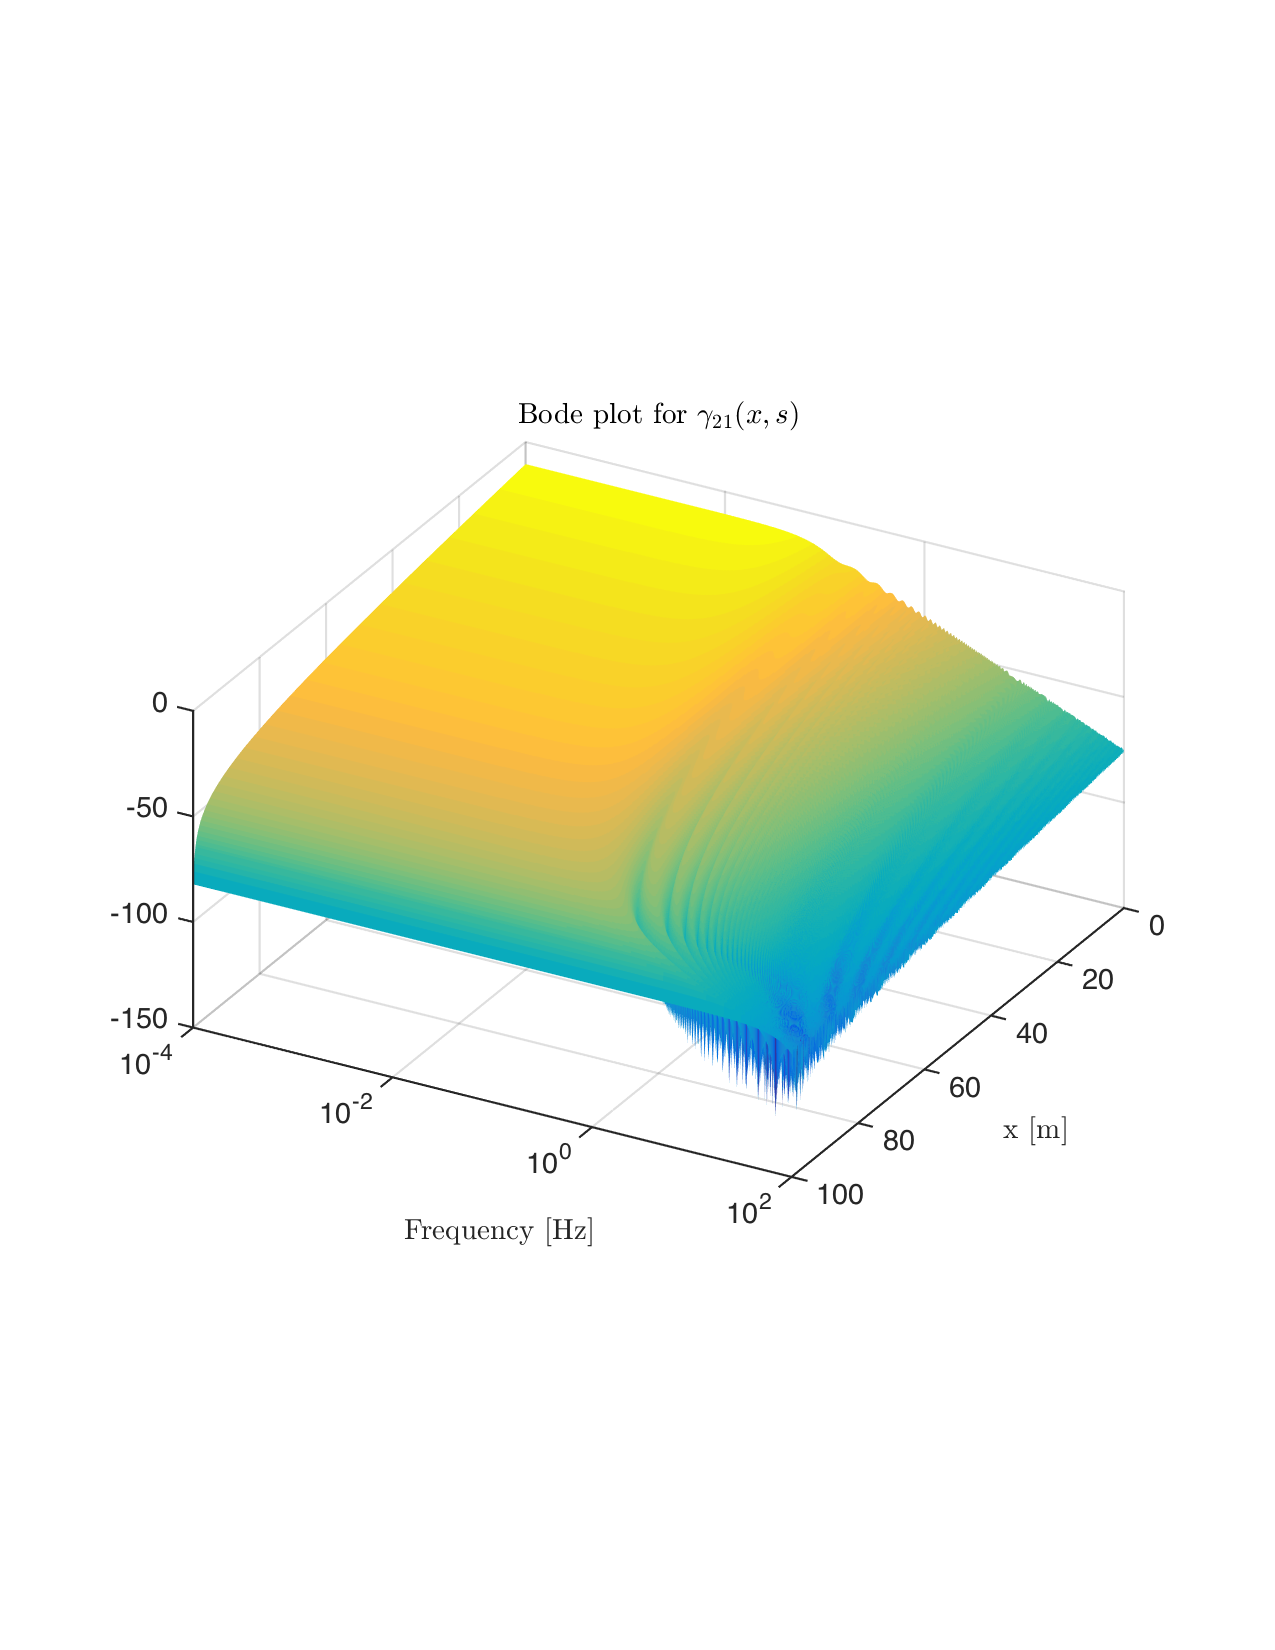
\includegraphics[trim = 0mm 60mm 0mm 60mm, width = 8cm]{distr_gamma_21}
%\tabularnewline
%Spatial magnitude Bode plot for $\gamma_{11}(x,s)$.
%&
%Spatial magnitude Bode plot for $\gamma_{21}(x,s)$.
%\tabularnewline
%\end{tabular}
%\caption{Spatial magnitude Bode plots for Riemann invariants in congested regime ($\left|\alpha\right| = $ 0.05 Hz)\label{fig:Magn_spatial_diag_congested}}
%\end{figure}

\begin{figure}
\centering
\begin{tabular}{cc}
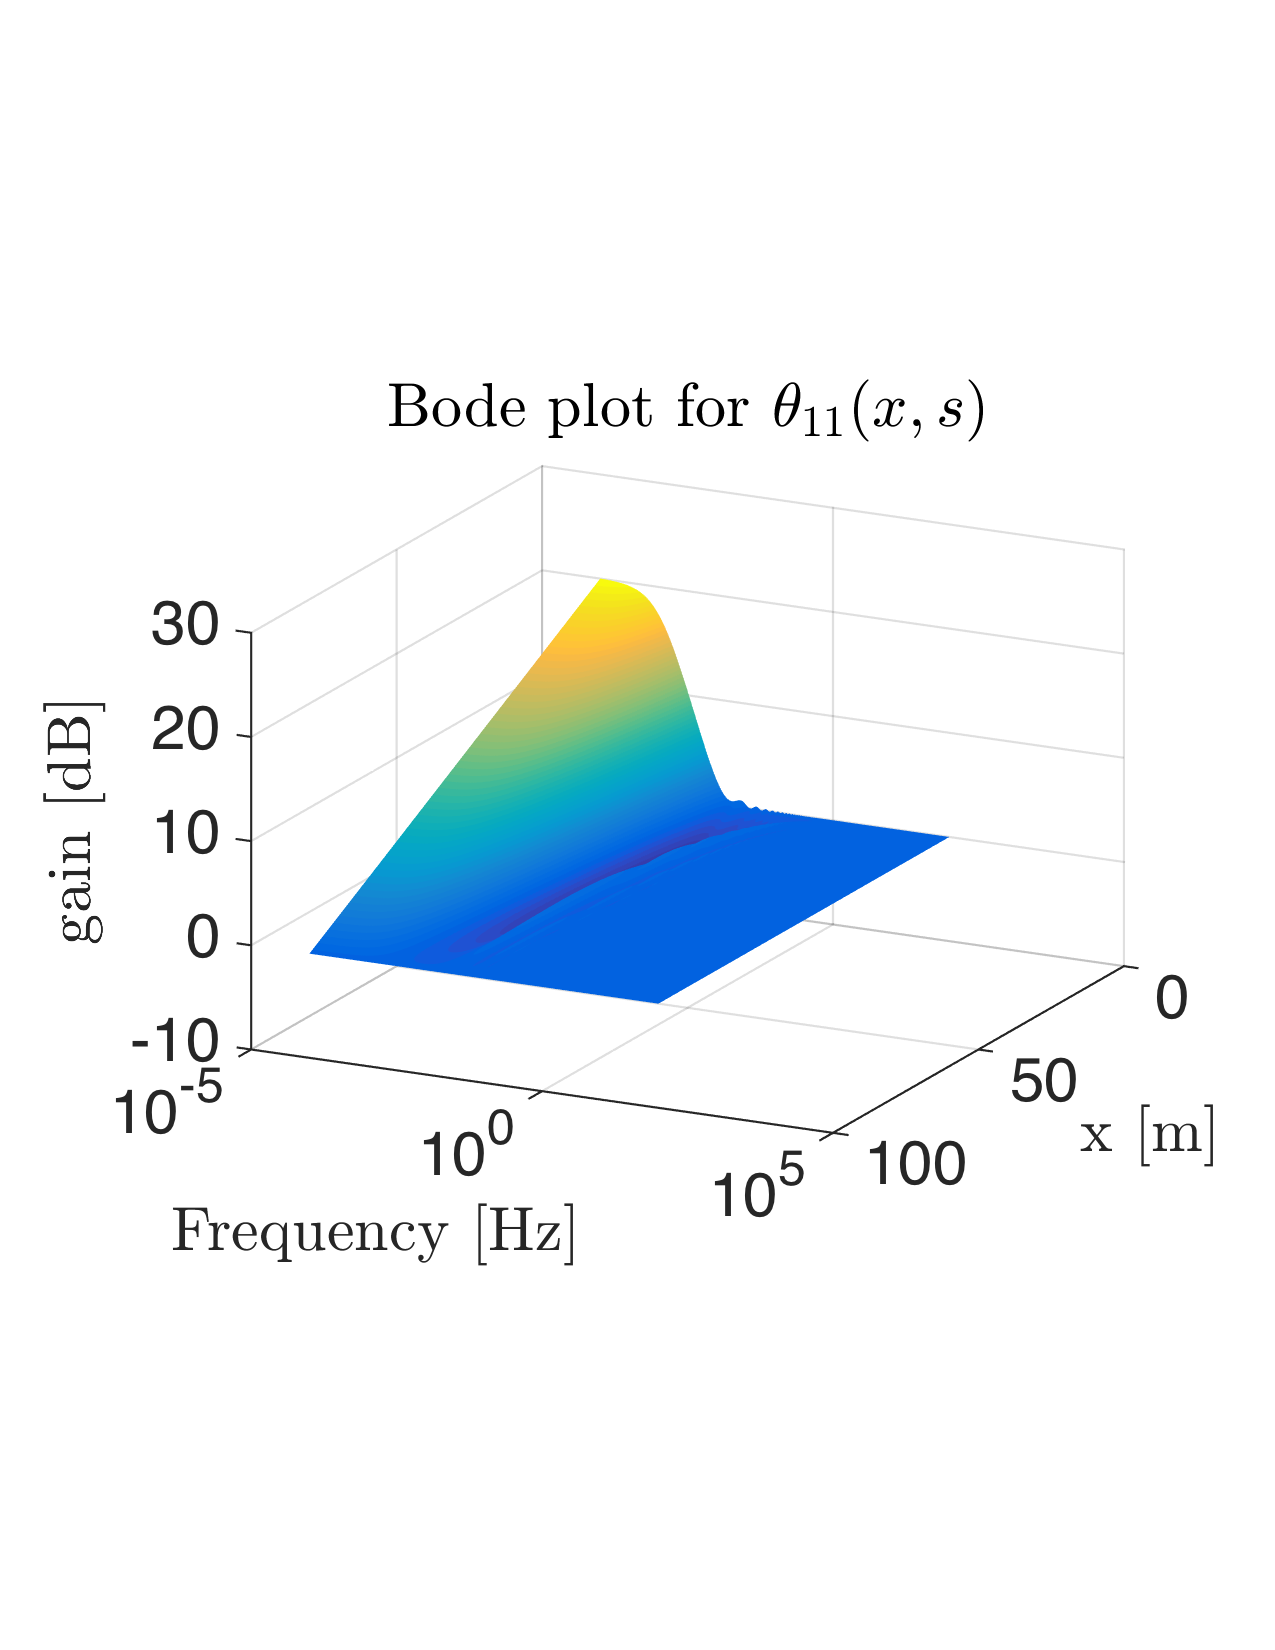
\includegraphics[trim = 0mm 60mm 0mm 60mm, width = 5cm]{distr_theta_11}
\tabularnewline
Spatial magnitude Bode plot for $\theta_{11}(x,s)$.
\tabularnewline
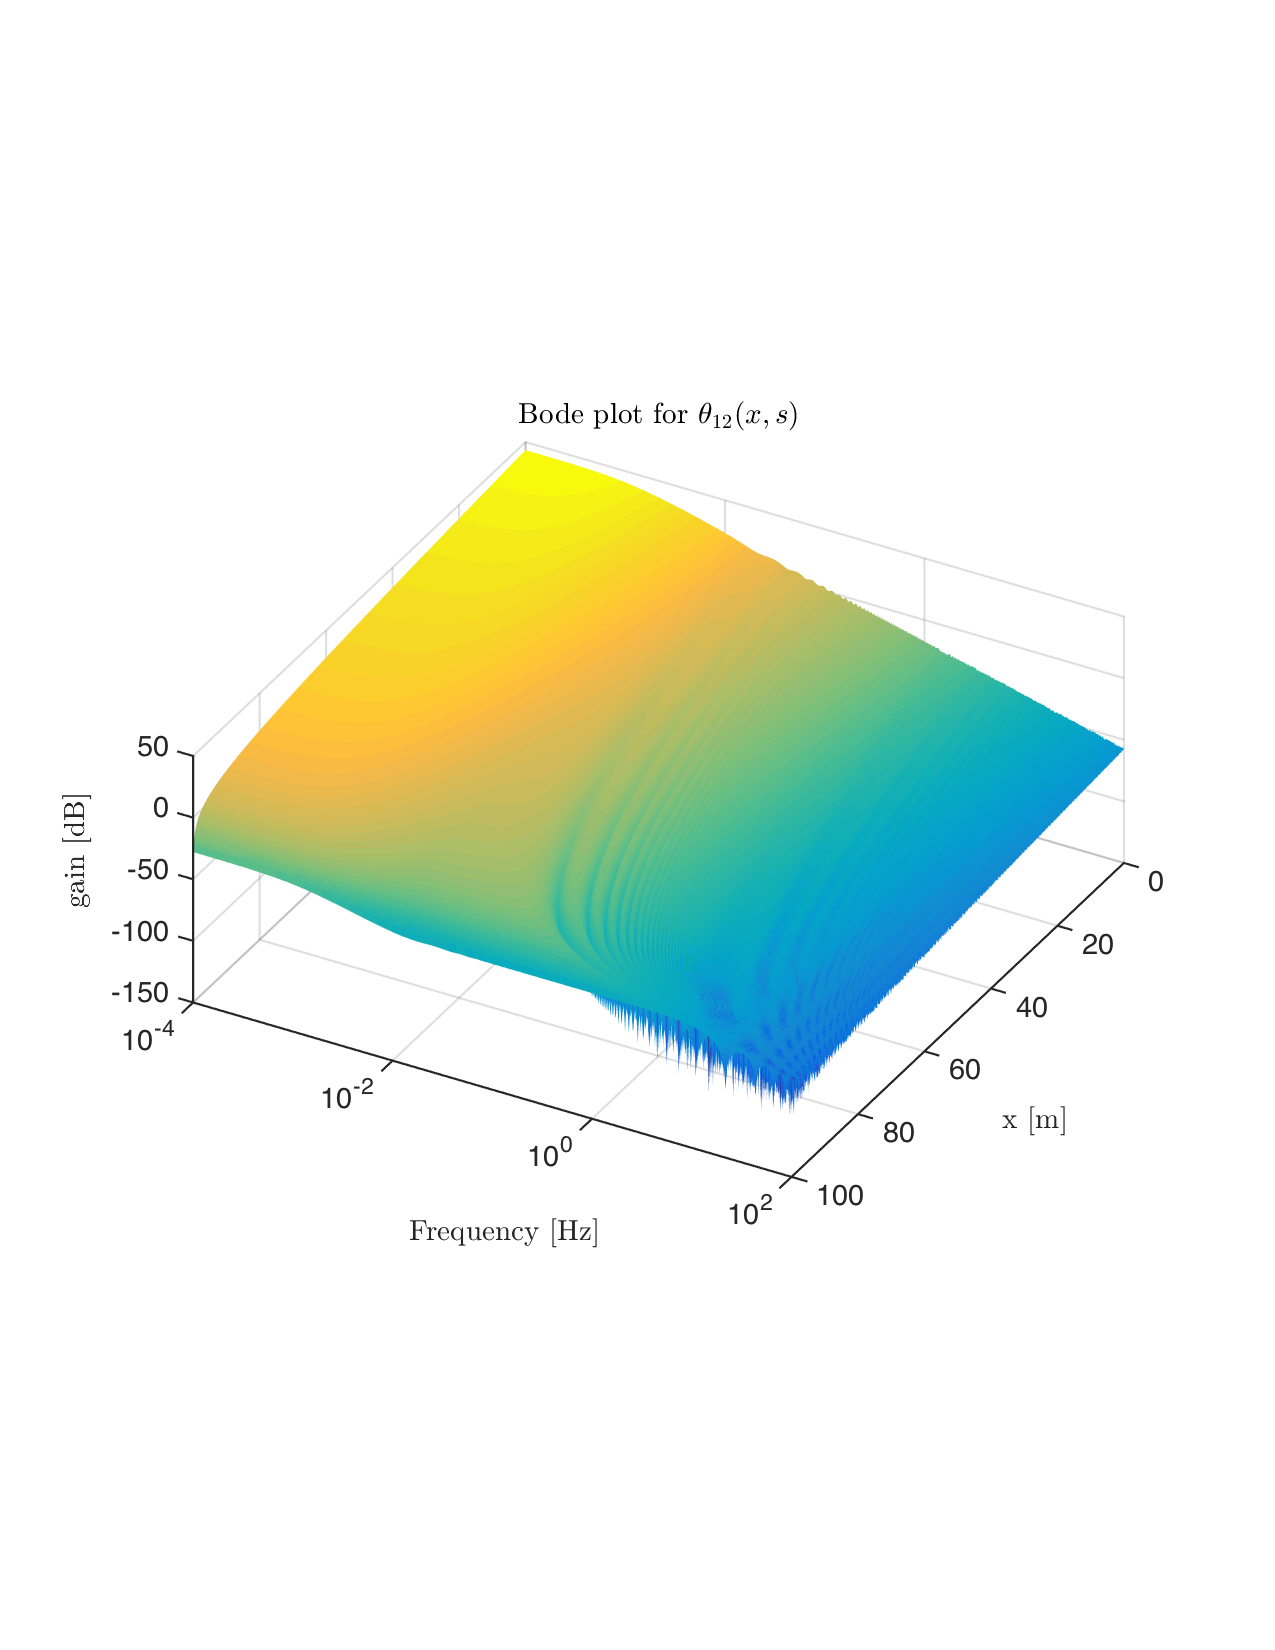
\includegraphics[trim = 0mm 60mm 0mm 60mm, width = 5cm]{distr_theta_12}
\tabularnewline
Spatial magnitude Bode plot for $\theta_{12}(x,s)$.
\tabularnewline
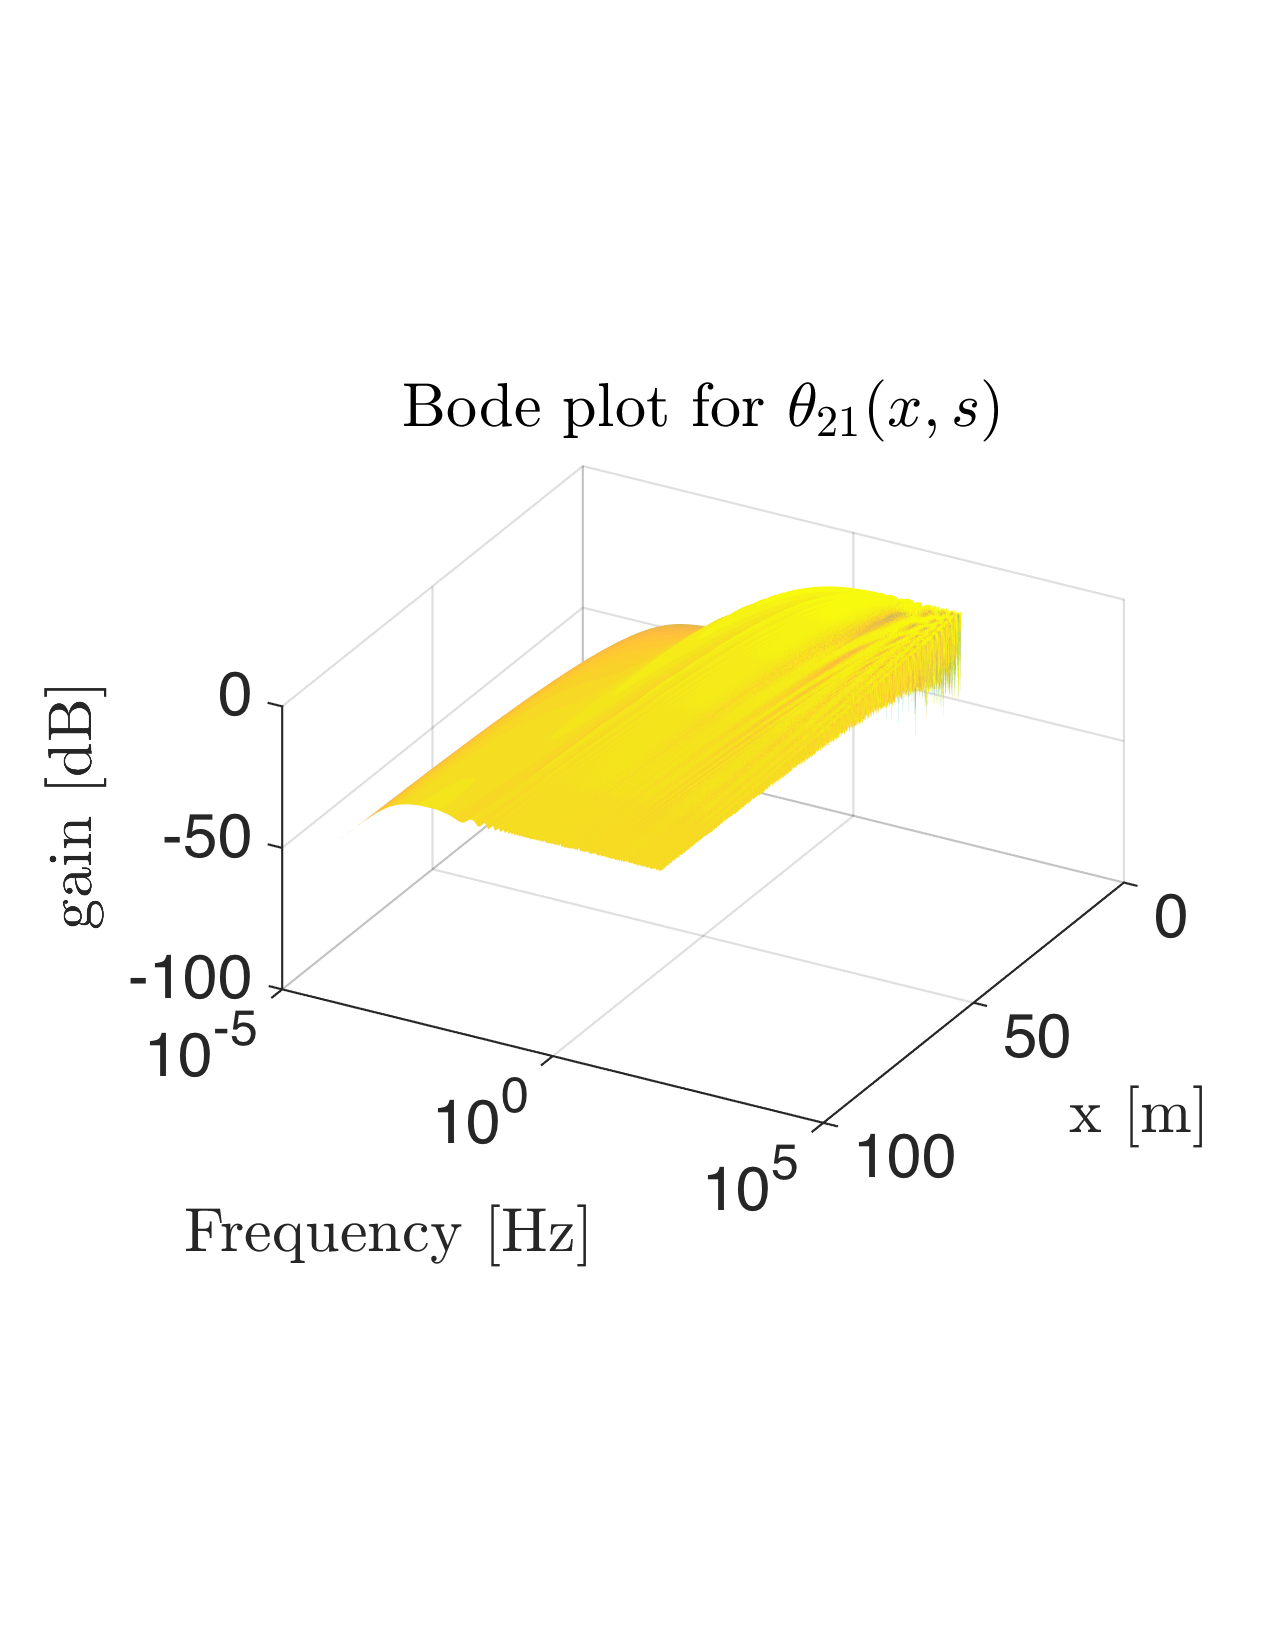
\includegraphics[trim = 0mm 60mm 0mm 60mm, width = 5cm]{distr_theta_21}
\tabularnewline
Spatial magnitude Bode plot for $\theta_{21}(x,s)$.
\tabularnewline
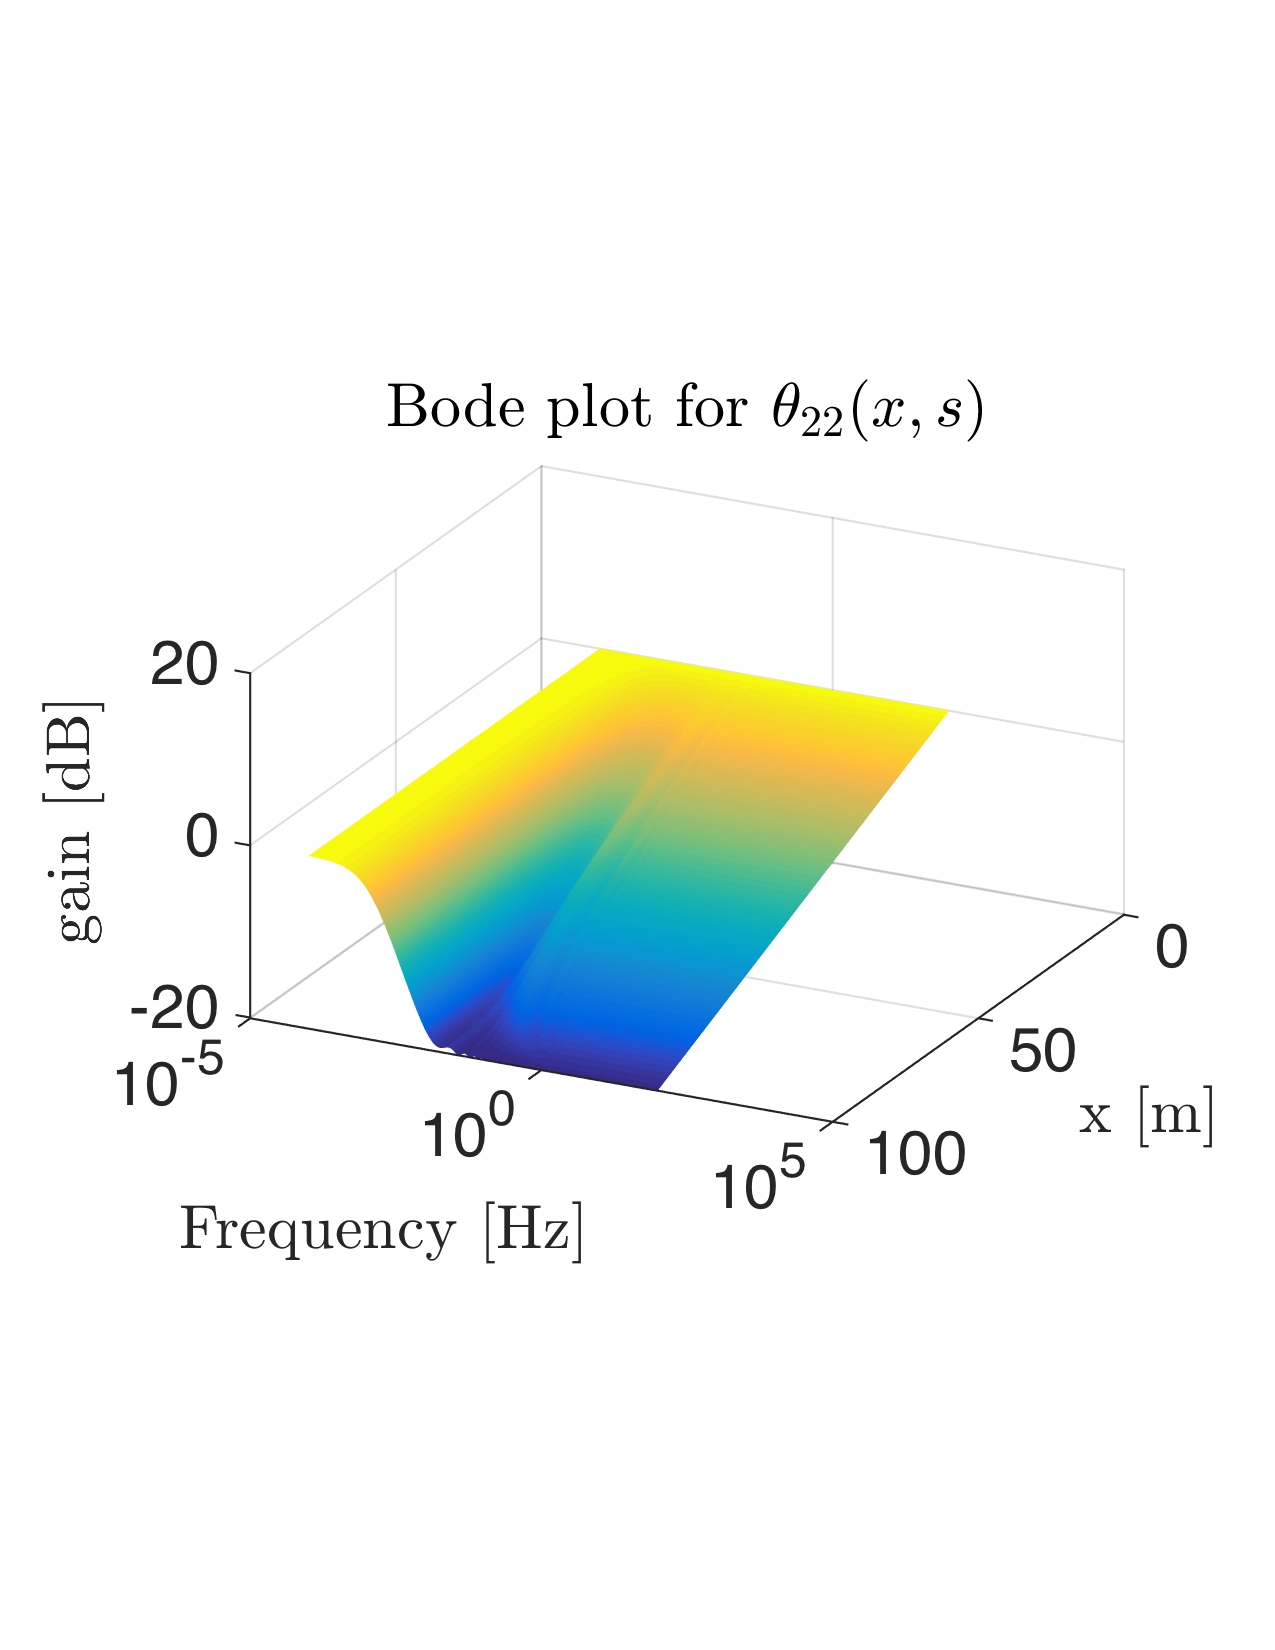
\includegraphics[trim = 0mm 60mm 0mm 60mm, width = 5cm]{distr_theta_22}
\tabularnewline
Spatial magnitude Bode plot for $\theta_{22}(x,s)$.
\tabularnewline
\end{tabular}
\caption{Spatial magnitude Bode plots for physical variables in congested regime ($\left|\alpha\right| = $ 0.05 Hz)\label{fig:Magn_spatial_physx_congested}}
\end{figure}

\subsubsection{Poles and BIBO stability of the system}
In order to practically assess the presence of poles, numerical search for roots of the denominator of the transfer functions has been conducted thanks to standard equation solvers. Once more $-\alpha$ is a solution and another one was found at $s=-0.0018$. They are both negative reals and therefore cannot make the system unstable. Although the solvers could have detected poles with a non zero imaginary part, none has been found. Holistic search for other poles should be conducted but is out of the scope of this article.

\subsection{Findings and conclusion from the theoretical study}
The numerical experiments above have validated the accuracy of the linearized model and highlighted several of its core properties.
\begin{itemize}
\item The TFN delineates two regimes: congested for $F > 1$ and free-flowing for $F < 1$. This classification, and the resulting stability result legitimize the use of linearization about a nominal point in the stable region.
\item  The assessment of convective instability in the free flow regime is of course applicable to this specific model (other models such as \cite{Jamitons-multi-valued-fund} might lead to other conclusions, and all need to be checked against experimental data). Here, exponential growth of the linearization error only occurs in a conic region of the  $\left[0,T\right] \times \left[0,L\right]$ domain where convective instability travels along the characteristics.
\item The absolute value of the term $\alpha = -\dfrac{\lambda_2}{\tau(\lambda_1 - \lambda_2)}$ is a characteristic frequency of the system. It delineates the low frequency domain in which approximate expressions help decompose the transfer functions in simple gain and delay components. In the spectral domain, $\lambda_{1}$ and $\lambda_{2}$ appear as information propagation speeds in distributed delay elements while  $\tau\lambda_{1}$ acts as the characteristic distance of distributed gain components.
%\item Low frequency analysis ($\left|s\right|\ll\left|\alpha\right|$) also highlighted that transfer functions between physical variables are structurally similar in free-flow and congested regimes. The only dissimilarities that arise in the approximate expressions are due to the fact that boundary conditions are not set at the same locations depending on whether the regime is congested or free-flowing.
\end{itemize}


\section{Numerical validation}

In this section we demonstrate the ability of the linearized ARZ equations to model the various nonlinear dynamics around a nominal operation point, The spectral form of the linearized
model provides a well-established control theoretic framework for designing control strategies for the system. Prior to using such techniques, it is necessary to assess how accurate the
model is in its linearized form. This section compares the prediction of the model with actual flow
and velocity data gathered from the well-known NGSIM data set.


\subsection{Data source: NGSIM trajectories}

We use the NSGIM trajectory data set for a section of the US-101 highway. The set gathers trajectories of vehicles sampled with a 10 Hz frequency thanks to high precision cameras. The data is pre-processed so as to take only cars into account; 45 minutes are recorded on a 650-meter long section with five lanes. The lanes are taken into account when computing the lineic density of vehicles $\rho$.
A map of the time evolution of speed along the section is given in Figure \ref{fig:NGSIM-trajectories}.
Only a subset of the spatial domain is used due to the presence of ramps, which breaks the homogeneity of the freeway. The viable domain is 200 meters long.

\begin{figure}[H]
\centering
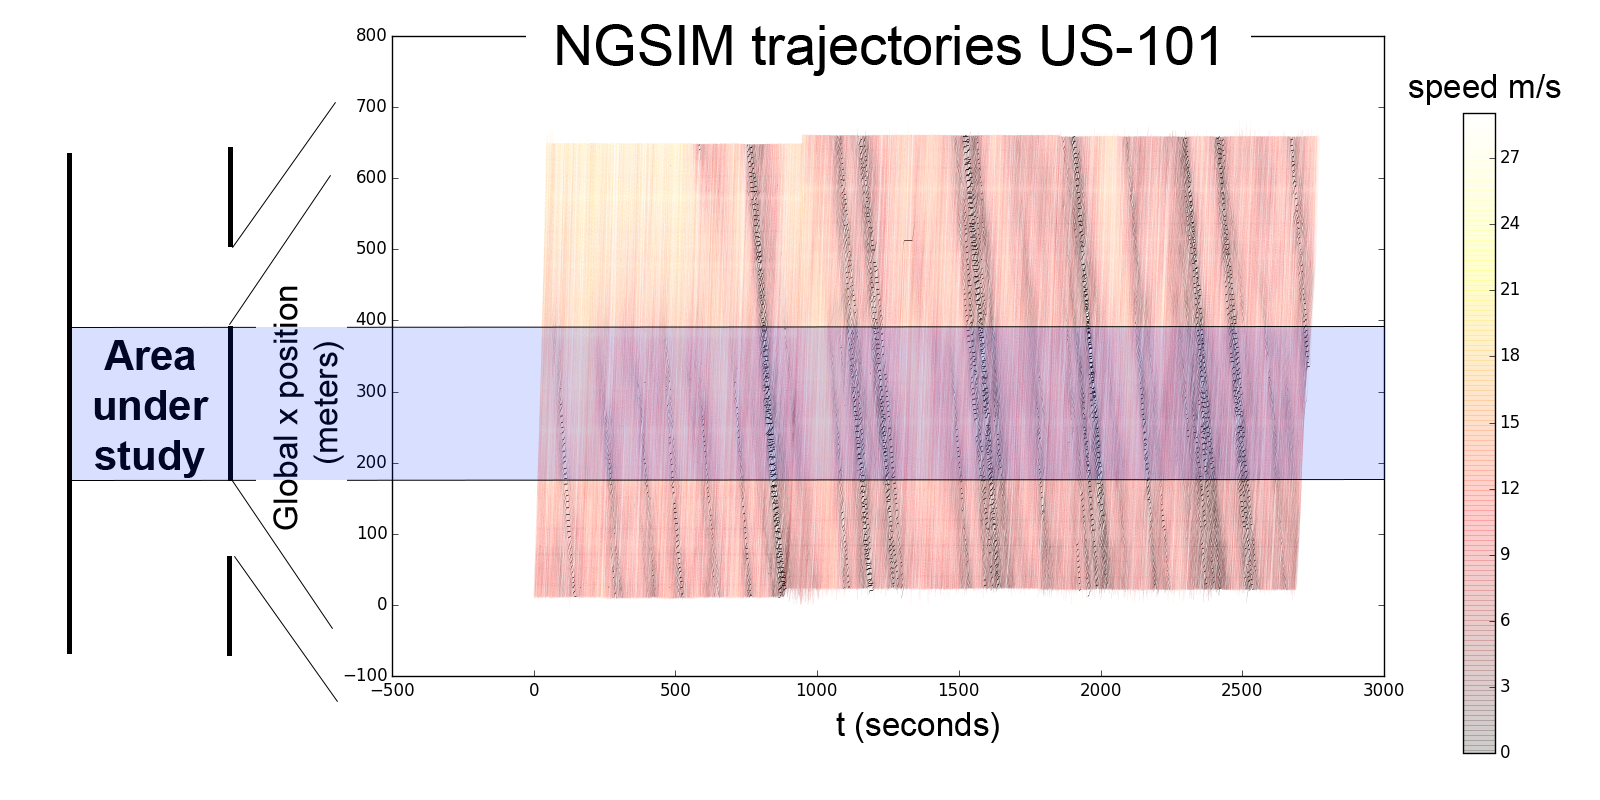
\includegraphics[width=8cm]{US-101_all_traj_low_res_mod}
\protect\caption{NGSIM trajectories. Color represents the measured speed of each
car in m/s.}
\label{fig:NGSIM-trajectories}
\end{figure}



\subsection{Reconstructing $(v,q)$ maps from NGSIM trajectories}

The NGSIM data set does not directly provide the values $v(t,x)$ and $q(t,x)$ in the resolution domain $\left[0,T\right]\times\left[0,L\right]$. To obtain macroscopic quantities out of the microscopic measurements, we follow the approach devised in \cite{edie1963discussion} and divide the space-time grid into cells $\left(\left[i\Delta t,\, \left(i+1\right)\Delta t\right]\times\left[j\Delta x, \, (j+1)\Delta x\right]\right)_{i\in\left\{ 1\ldots n_{t}\right\} ,j\in\left\{ 1\ldots n_{x}\right\} }$, where $n_t$ and $n_x$ are the number of cells in time and space, respectively. We denote each cell as $\bin_{i,j}$. This operation consists of gathering corresponding data points into cells, then estimating the quantities of interest in each cell, it was for example used in \cite{Piccoli201532}.

Within each cell, a specific number of traces, or footprints of a vehicle along its trajectory, are available, and $\rho$, $v$, and $q$ are assumed to be constant. We present several formulae to map a set of traces to speed, flow, and density over the space-time grid. 

\textbf{Binning formula for $v$}: Since the speed is assumed to be constant in each cell, a straightforward estimate for the speed is the empirical average. The estimator for $v$ in $\bin_{i,j}$ is

\begin{equation}
\widehat{v}_{i,j}=\mean_{\trc \in \bin_{i,j}}(v(\trc)).
\end{equation}

\textbf{Binning formula for $\rho$}: By definition, the density of $\bin_{i,j}$ is  
\begin{equation}
\rho_{i,j}=\frac{1}{n_{\lns}\Delta x\Delta t}\iint_{\left(t,x\right)\in [i\Delta t, \,(i+1)\Delta t] \times [j\Delta x,\,(j+1)\Delta x]}\rho(x,t) \text{d}x \text{d}t.
\end{equation}

The position of each vehicle is recorded every 0.1 second. For each cell we count the number of traces and normalize it by the sampling rate. The contribution of a given vehicle to the density of a cell is proportional to the number of traces it has left in the cell. If the speed is assumed to be locally constant, this contribution is proportional to the time this vehicle spends in the cell and is consistent with the conservation of the total number of vehicles across all cells. Then we have the density estimator
\begin{equation}
\widehat{\rho}_{i,j}=\frac{1}{n_{\lns} \Delta x \Delta t \: \text{sampling rate}}\card ( \{ \trc \mid \trc \in \bin \} ),
\end{equation}
where $\card (\cdot)$ gives the number of elements in a set, i.e., its cardinal. 

\textbf{Binning formula for $q$}: By definition, $q=\rho v$, so a logical first estimate for $q$ in $\bin_{i,j}$ is 
\begin{equation}
\widehat{q}_{i,j}=\widehat{v}_{i,j}\widehat{\rho}_{i,j}.
\end{equation}

We can also approximate the flux through $\bin_{i,j}$ with a simple counting method. If a vehicle crosses spatial coordinate $\left(j+1\right)\Delta x$ between times $i\Delta t$ and $\left(i+1\right)\Delta t$, then it leaves a trace in both $\bin_{i,j}$ and $\bin_{i,j+1}$. Counting these vehicles and normalizing by the duration $\Delta t$ gives the estimator
\begin{equation}
\widehat{q}_{i,j}^{\cnt}=\frac{1}{n_{\lns}\Delta t}\: \card\left(\left\{ \text{id} \left(\trc\right)\mid \trc \in \bin_{i,j}\right\} \cap\left\{ \text{id}\left( \trc \right)\mid \trc\in \bin_{i,j+1}\right\} \right),
\end{equation}
where id$(\cdot)$ gives the identification number of a vehicle.



\subsubsection{Choosing the number of bins}

As the estimation formulae above rely on averaging, having a comfortable
number of points in each bin provides more stable estimates. It is worth mentioning that usual central limit theorem based reasoning for convergence of such estimates is flawed as several samples may correspond to the same vehicle or interacting vehicles, violating the independence assumption of the theorem. Proving the convergence of the estimates above lies beyond the scope of this article. As a rule of thumb we choose a discretization that guarantees that most bins will host more than $100$ traces. This is achieved with a $80\times80$ grid where the $10^{\text{th}}$ percentile of the number of traces in a given bin is $170$. Such a grid also yields a $10^{\text{th}}$ percentile of $56$ distinct vehicles per bin. 

%The histograms of number of traces and vehicle per cell are given in Figure \ref{fig:Grid control}.

%\begin{figure}[H]
%\centering
%\begin{tabular}{cc}
%\includegraphics[width=6cm]{\string"traces_80_80\string".png} & \includegraphics[width=6cm]{\string"ids_80_80\string".png}\tabularnewline
%Histogram of number of traces per cell. & Histogram of number of distinct vehicles per cell. \tabularnewline
%\end{tabular}
%\caption{Experimental justification for a $80\times 80$ cell based discretization
%grid for the NGSIM data.}
%\label{fig:Grid control}
%\end{figure}

While our goal here is not to present theoretical proofs of the convergence of the binned estimators for $\left(v,\rho,q\right)$, it is nonetheless possible to check that the procedure is coherent. Two estimators are provided for $q$ that use radically
different techniques: the first relies on the average measured speed and the number of traces in a bin, while the other relies on counting vehicles transiting from a cell to another. Figure \ref{fig:Sanity-check} show that the scatter plot of $\widehat{q}_{i,j}^{\cnt}$ plotted against $\widehat{q}_{i,j}$ coincides nicely with the line $y=x$, validating the overall binning and estimation procedure above.

\begin{figure}[H]
\centering
\includegraphics[width=6cm]{\string"80_80_q_q_count\string".png}
\protect\caption{Sanity check for the estimation procedure. $\widehat{q}_{i,j}^{\text{count}}$
is plotted against $\widehat{q}_{i,j}$ across the grid of bins.
\label{fig:Sanity-check}}
\end{figure}



\subsection{Estimated values for $\left(v,q\right)$} 

To check how well the linearized ARZ model fits an actual dataset, we chose a bounded domain and compare the theoretical solution given by the second-order model and the observed data. Again we focus on the variables $v$ and $q$. Using the estimation procedure above, we compute fundamental diagrams from which we estimate the eigenvalues $\lambda_{1}$ and $\lambda_{2}$.
To calibrate the relaxation time $\tau$, we analyze the errors of predicted values of $v$ and $q$ for various $\tau$. The resulting maps of both the predicted and observed values highlight phenomena that the linearized model can and cannot account for. 

\textbf{Maps.} The estimates $\widehat{v}_{i,j}$, $\widehat{\rho}_{i,j}$, $\widehat{q}_{i,j}$, and $\widehat{q}_{i,j}^{\text{count}}$ are plotted on the discretized grid in Figure \ref{fig:Estimated-values}. Note that $\widehat{q}$ and $\widehat{q}^{\text{count}}$ give extremely similar results, so we may use $\widehat{q}^{\text{count}}$ from this point on. Damped oscillations and smoothly decaying values along characteristic lines are the main characteristic the practical implementation of the model should feature.

\textbf{Fundamental diagrams.} From the estimated values we can easily compute the fundamental diagrams given in Figure \ref{fig:Empirical-fundamental-diagrams}. We use the fundamental diagrams to calibrate the model parameters. Though the dataset used is dense, it covers only a small region of time and space. Thus, its small size is a potential flaw in our model parameter calibration as it is certain that
our measurements are highly correlated. This seems
to be confirmed by the fact that the fundamental diagrams below correspond only to the congested regime. \
%textit{OPTIONAL: Most of the points are concentrated
%about the same region. This is not enough to guarantee that the estimated
%quantities are reliable. However, NGSIM is to this day one of the
%most comprehensive data sets of vehicle behavior on a freeway. It
%is therefore one of the best ways one has to validate that a traffic
%model is realistic. The fact that most points lie in the same region
%is also a sign that the linearization hypothesis is reasonable
%in that context. Observed deviations from the equilibrium are indeed
%generally small. (The equilibrium, i.e. the linearization point, is estimated
%below).}

%\begin{figure}[H]
%\centering
%\begin{tabular}{cc}
%\includegraphics[width=8cm]{\string"80_80_v_map\string".png} & \includegraphics[width=8cm]{\string"80_80_rho_map\string".png}\tabularnewline
%\includegraphics[width=8cm]{\string"80_80_q_map\string".png} & \includegraphics[width=8cm]{\string"80_80_q_count_map\string".png}\tabularnewline
%\end{tabular}
%\protect\caption{Estimated values for $\left(v,q,\rho\right)$. Top left: $\widehat{v}_{i,j}$.
%Top right: $\widehat{\rho}_{i,j}$. Bottom left: $\widehat{q}_{i,j}$.
%Bottom right: $\widehat{q}_{i,j}^{\text{count}}$ .\label{fig:Estimated-values}}
%\end{figure}

\begin{figure}[H]
\centering
\begin{tabular}{ccc}
\includegraphics[width=5cm]{\string"80_80_fundamental_diagram_rho_q_count\string".png} & \includegraphics[width=5cm]{\string"80_80_fundamental_diagram_v_q_count\string".png} & \includegraphics[width=5cm]{\string"80_80_fundamental_diagram_v_rho\string".png}\tabularnewline
\end{tabular}
\protect\caption{Empirical fundamental diagrams. Left: $\left(\widehat{\rho},\widehat{q}^{\text{count}}\right)$.
Middle: $\left(\widehat{v},\widehat{q}^{\text{count}}\right)$. Right: $\left(\widehat{\rho},\widehat{v}\right)$.
\label{fig:Empirical-fundamental-diagrams}}
\end{figure}


\textbf{Calibration of $\lambda_{1}$ and $\lambda_{2}$, linearization point.} In Section \ref{ARZSection}, we found that $\lambda_{1}$ is exactly $v^*$ and $\lambda_{2}$ is the slope of the fundamental diagram at $v^*$. Thus to calibrate the eigenvalues we must find the linearization point. We estimate the linearization point using the Ordinary Least Squares method. Note the dataset used corresponds only to the congested regime and the fundamental diagram is almost affine. The estimator, $\widehat{\lambda}_1=\widehat{v}^*$ is chosen as the empirical mean of $\widehat{v}_{i,j}$. To estimate $\lambda_{2}$, we fit a linear model $\widehat{q}^{\text{count}}=b_{1}\widehat{\rho}+b_{0}+\varepsilon$, where $\varepsilon$
represents the noise in the model that would ideally be centered,
homoschedastic, and uncorrelated but is not practically. Then $\widehat{\lambda}_{2}=\widehat{b}_{1}$ and we take $\widehat{q}^*$ as the empirical average of $\widehat{q}^{\cnt}$. The ratio of $\widehat{q}^*$ and $\widehat{v}^*$ gives the estimate $\widehat{\rho}^*$.
Provided each estimator is convergent, the continuity of the functional
$\left(x,y\right)\rightarrow\frac{x}{y}$ on its domain guarantees the convergence of $\widehat{\rho}^*$. The empirical results are presented in Figure \ref{fig:Calibration-of-eigen-values}. The determination coefficient is poor but can be improved by filtering out outliers and gathering more data. Future work should include improving the quality of the estimation. Significance tests for the coefficients of the linear model are not presented. The assumptions they rely on about
the linear dependency between $\widehat{q}$ and $\widehat{v}$ are clearly
not respected here as the noise is auto-correlated. Further work should also turn this rather heuristic method for estimating parameters
into a fully justified statistical procedure. Note that the goal of the present article is to provide a new model and corresponding spectral analysis, which we want to illustrate with state of the art data. Thus, development of statistical methods to handle this data is out of the scope of the present investigation.

\begin{figure}[H]
\centering
\includegraphics[width=6cm]{\string"Fundamental_diagram_fitting_n_80\string".png}
\protect\caption{Calibration of $\lambda_{1}$ and $\lambda_{2}$. The circle denotes the linearization point. The affine model used to estimate $\lambda_{2}$ and the linearization point is also plotted. The estimates are: $\widehat{\lambda}_{1}=8.96$ m/s, $\widehat{\lambda}_{2}=-4.37$ m/s, $\widehat{\rho}^{*}=0.049$ veh/m, $\widehat{v}^{*}=8.96$ m/s, $\widehat{q}^{*}=0.44$ veh/s, with $r^{2}=0.48$. The characteristic frequency of the system is $\widehat{\alpha} = 8.37\times10^{-3}$ Hz. Its order of magnitude does correspond to practical traffic flow modeling.}
\label{fig:Calibration-of-eigen-values}
\end{figure}

\subsection{Verification of the spectral form}
In this section we demonstrate the performance of the spectral form as a prediction tool using the time domain responses derived from the transfer functions (see \ref{sub:Generic-computations}) and FFT. Since we are working with a linearized system, we can decompose boundary conditions then add predicted values inside the domain $\left[0,T\right]\times\left[0,L\right]$. Fourier decomposition of boundary conditions is here extremely accurate as the median relative errors for the interpolation of the values of $\xi_{1}\left(x=0, \cdot \right)$ and $\xi_{2}\left(x=L, \cdot \right)$ are respectively $2\%$ and $3\%$.
%A real signal $\left\{ f\left(t\right)\mid t\in\left[0,T\right]\right\} $ on one of the boundaries $\left\{ \left(x=0,t\right)\mid t\in\left[0,T\right]\right\} $ or $\left\{ \left(x=L,t\right)\mid t\in\left[0,T\right]\right\} $ is transformed into a periodic signal by infinite duplication and then turned into a Fourier series $\left\{ t\rightarrow\mu+\sum_{k=1}^{n}\beta_{k}\cdot \left(k\cdot wt+\phi_{k}\right)H\mid t\in\left[0,T\right]\right\} $. This process is known to be convergent with an infinite sum for any square integrable function. It is practically extremely accurate in our case even though the FFT only relies on a finite number of Fourier coefficients. 


\textbf{Simulated maps.} Since the spectral form presents information in the diagonalized basis, we need a conversion before we can compare the simulated results to the values estimated from the dataset.  
To make a comparison in the diagonalized basis, we first compute the estimated deviations from the equilibrium $\widehat{\widetilde{v}}_{i,j}=\widehat{v}_{i,j}-\widehat{v}^{*}$ and $\widehat{\widetilde{q}}_{i,j}=\widehat{q}_{i,j}-\widehat{q}^{*}$. Then the estimates for $\xi_{1}$ and $\xi_{2}$ are given by $\widehat{\xi}_{1_{i,j}}=\frac{\widehat{\rho}^{*}\widehat{\lambda}_{2}}{\widehat{\lambda}_{1}-\widehat{\lambda}_{2}}\widehat{\widetilde{v}}_{i,j}+\widehat{\widetilde{q}}_{i,j}$ and
$\widehat{\xi}_{2_{i,j}}=\frac{\widehat{\rho}^{*}\widehat{\lambda}_{1}}{\widehat{\lambda}_{1}-\widehat{\lambda}_{2}}\widehat{\widetilde{v}}_{i,j}$. To compare the physical variables, we compute the velocity and flow predictions by inverting \eqref{eq:Riemannzeta}: $\widetilde{q}=\xi_{1}-\frac{\lambda_{1}}{\lambda_{2}}\xi_{2}$,
$\widetilde{v}=\frac{\lambda_{1}-\lambda_{2}}{\rho^{*}\lambda_{1}}\xi_{2}$.

Figure \ref{fig:Data-versus-predicted.} shows important qualitative properties of the model. As expected, the model generally predicts with very good accuracy the decay of all quantities along their characteristic lines, a realistic feature that cannot be paralleled by first-order models. The general quality of the fit is rather good with most of the error on $v$ and $q$ in a $20\%$ range of the data's amplitude between minimum and maximum values. Furthermore the linearized second-order model manages to capture oscillations observed on the boundary and account for their decay accurately. 

\textbf{Calibration of $\tau$\label{sub:Calibration-of-tau}} For each $\tau$ we compute the \textit{mean absolute error} (MAE), or the average difference in absolute value between simulated and predicted values for each discretization cell. Since the quantities $v$ and $q$ are not physically homogeneous, it is not sensible to aggregate the errors over these quantities. However, $\xi_{1}$
and $\xi_{2}$ are both expressed in veh/s. Summing their MAE gives a reliable uni-dimensional index of the quality of the fit with respect
to $\tau$. This quantity is computed for different values of $\tau$
ranging from 5 to 80 seconds. The value offering the best fit
is $\tau^{*}=39.18$ s.

\begin{figure}[H]
\centering
\begin{tabular}{c}
\includegraphics[width=15cm]{\string"vq_map_n_80_best_tau\string".png}\tabularnewline
\includegraphics[width=15cm]
{\string"xi_map_n_80_best_tau\string".png}
\end{tabular}
\protect\caption{Data versus predicted. Top Figure: $\left(v,q\right)$ domain, top row is $v$, bottom row is $q$. Bottom: $\left(\xi_{1},\xi_{2}\right)$
domain, top row is $\xi_{1}$, bottom row is $\xi_{2}$. First column: data. Middle column: predictions. Third column: error (difference between prediction and data).\label{fig:Data-versus-predicted.}}
\end{figure}

\begin{figure}[H]
\centering
\begin{tabular}{cc}
\includegraphics[width=8cm]
{\string"q_v_error_80\string".png} 
& \includegraphics[width=8cm]{\string"xi_1_xi_2_error_80\string".png}\tabularnewline
MAE over $q$ and $v$ & MAE over $\xi_{1}$ and $\xi_{2}$ and sum of both MAE.\tabularnewline
\end{tabular}
\protect\caption{Calibration of $\tau$, one minimizes the sum of MAE over $\xi_{1}$
and $\xi_{2}$.}
\end{figure}


\subsection{Findings and conclusion from the numerical experiments}
The numerical experiments above have validated the accuracy of the linearized model and highlighted several of its core properties.
\begin{itemize}
\item The numerical experiments above show that the linearized ARZ model is capable of reproducing NGSIM data accurately for a homogeneous segment of the US-101 freeway. Oscillations are accounted for as well as their damping delay.
\item The spectral approach provided here supports a solution to the underlying traffic flow model. In other words, the contribution of the work is to show that the model can support oscillatory behavior (through periodic solutions). This is the main difference with purely data driven approaches such as \cite{Zheng2011} for example.
\end{itemize}


\section{Conclusion}

As the full nonlinear ARZ equations have no known closed form solutions in the general case, they are difficult to analyze. The linearized equations enable the use of spectral methods presented here, allowing for elegantly simple yet powerful analysis tools relying on explicit solutions. These equations are diagonalized, and solved explicitly using a spectral representation (distributed transfer function). Using this approximation, we are able to analyze them around a nominal flow and characterize the oscillatory behavior of the solution. The linearized model is able to capture important features of the flow which first order models cannot. 

With the linearized ARZ model, we were also able to define the Traffic Froude Number $F$. This quantity is computed using the eigenvalues of the system and characterizes the flow regime of the road section under consideration.

%We found the eigenvalues of the linearized system to be constant, prompting the definition of the Traffic Froude Number, $F$, which indicates the flow regime of the road section under consideration. Note that the Froude number inequalities delineating the supercritical and subcritical regimes in hydronamics are reversed for our definition of the TFN. 

Considering the transfer function of the linearized system of equations delineates the conditions for stability of the approximation about the equilibrium. The time domain responses we derive show that the system is unstable when one of the eigenvalues is negative. In the free-flow regime, $F < 1$, values of flow and speed increase exponentially in a conic region of space and time and the system leaves the linear regime, while in the congested regime, $F>1$, oscillations decrease. In the latter case, the system remains in the linear regime and oscillations on boundary conditions are damped with an exponential rate along the characteristic lines. Thus, the TFN is also an indicator of linear stability.

The behavior predicted in congested regime for traffic does not present shocks and Fourier spectral analysis cannot account for more nonlinear and non-smooth behavior as well as wavelet transforms. However, our spectral domain study paves the way to applying standard linear system control theory to traffic, with a linearized second model that is empirically reliable in terms of reproducing actual data. Future work will therefore focus on controller design based on the spectral framework presented here.

%The present analysis also complements the wavelet-based approach used in \cite{Zheng2011}. Fourier transform based analysis is a powerful tool in our numerical experiments that does not require any CFL-like condition for stability. The linearity of the system clearly predicts smoother behavior than what is found with wavelet decomposition, and as we have shown, the resulting macroscopic predictions are fairly accurate.


%Second order models, because of their inherent complexity, were hard to analyze so far. No closed form solution was available and the frequency domain responses could not be written explicitly. Although it only offers an approximate representation of the system, our linearizing about an equilibrium has enabled a powerful yet simple analytical foundation for analysis. In particular, we have shown how to characterize important properties of the system such as Riemann Invariants and the \textit{Traffic Froude Number} that separates two classes of behaviors solutions to the ARZ equation can follow.
%
%For the free flowing regime ($F>1$), we have shown that around the linearization point, traffic systematically features oscillations of exponentially increasing amplitude that drive the system away from its equilibrium. This conclusion is different from those of \cite{Flynn09self-sustainednonlinear, Jamitons-multi-valued-fund}. Indeed, no assumption is made about the structure of the fundamental diagram except for the fact that the equilibrium speed decreases with traffic density. The oscillations we find occur for densities below a threshold whereas Jamitons are predicted to appear when the traffic density lies above a critical point whose value depends on the shape of the fundamental diagram. In such a regime, oscillations systematically propagate downstream whereas Jamiton waves can propagate upstream.
%
%In congested regime ($F<1$), traffic oscillations are damped with an exponential rate equal to $\tau$. This guarantees the linearized solution remains about the equilibrium around which the approximate system is accurate. Although decaying slowly, the solution does not feature the rapid dissipation that makes first order models somewhat inaccurate. In our numerical experiments, the linearized second order ARZ model provably accounts for phenomena that CTM based models could not represent. Indeed, the latter predict fast dissipative convergence of traffic density towards a homogeneous quantity along the freeway section under scrutiny which does not correspond to the NGSIM measurements.
%
%The present analysis also complements the wavelet-based approach used in \cite{Zheng2011}. Fourier transform based analysis is arguably a powerful tool in our numerical experiments that does not need any CFL-like condition to guarantee accuracy of predictions. Transfer functions provide simple analytical expression that are easy to interpret in both free flowing and congested regimes. The linearity of the system clearly predicts smoother behavior than what is found with wavelet decomposition. The resulting macroscopic predictions are practically accurate as we have shown.
%
%To conclude, we find that a freeway section evolves as a classical linear system therefore exploding, oscillating or converging towards $0$ at an exponential rate. Linearization has enabled the translation of the ARZ model from cumbersome non-linear PDE derivations towards a simple set of equations readily usable for control. Designing the corresponding schemes to alleviate congestion will be the subject of our further work.

%\section*{Acknowledgments}
%The authors wish to thank Dr. Nikolaos Bekiaris-Liberis and Pierre-Olivier Lamare (PhD student at laboratoire Jean Kuntzmann) for their support in the first steps of adapting the spectral method from the Saint-Venant equation framework to the ARZ model. Professor L. Craig Evans' help has been extremely precious in understanding core theoretical properties of the linearized ARZ equations. The authors are also grateful to Dr. Guillaume Costeseque for his insightful comments on the draft.

%\section*{Appendices}
%\begin{itemize}
%\item Time domain solutions $(v, q)$
%\item Frequency domain for $(\rho, q)$, $(\rho, v)$
%\item Pre-processing of data
%\end{itemize}

\bibliography{biblio}

\end{document}
